% !Mode:: "TeX:UTF-8"
\documentclass[newtxmath=true,newgeometry=two,capcenterlast=true,subcapcenterlast=true,openright=true,library=false,absupper=true,fontset=windowsnew,type=master]{hithesis}
% 此处选项中不要有空格
%%%%%%%%%%%%%%%%%%%%%%%%%%%%%%%%%%%%%%%%%%%%%%%%%%%%%%%%%%%%%%%%%%%%%%%%%%%%%%%%
% 必填选项
% type=doctor|master|bachelor
%%%%%%%%%%%%%%%%%%%%%%%%%%%%%%%%%%%%%%%%%%%%%%%%%%%%%%%%%%%%%%%%%%%%%%%%%%%%%%%%
% 选填选项(选填选项的缺省值已经尽可能满足了大多数需求,除非明确知道自己有什么
% 需求)
% glue=true|false
% 	含义:由于我工规范中要求字体行距在一个闭区间内,这个选项为true表示tex自
% 	动选择,为false表示区间内一个最接近版心要求行数的要求的默认值,缺省值为
% 	false。
% tocfour=true|false
% 	含义:是否添加第四级目录,只对本科文科个别要求四级目录有效,缺省值为
% 	false
% fontset=siyuan|windowsnew|windowsold
% 	含义:注意这个选项视为了解决特殊问题而设置,比如用有些发行版本的linux排
% 	版时可能(大多数发行版不会)会遇到的字体无法载入的问题,或者字体载入之
% 	后出现无法复制的问题以及想要解决排版如 biang biang 面的 biang 这类中易
% 	宋体无法识别的汉字的问题。没有特殊的需要不推荐使用这个选项。
%
% 	如果是安装了 windowns 字体的 linux 系统,可以填写windowsnew(win vista
% 	以后 的字体)或 windowsold(vista 以前)或者想用思源宋体并且是已经安装
% 	了思源宋体的任何系统,填写siyuan选项。缺省值为空,自动识别系统并匹配字体
% 	。模板版中给出的思源字体定义文件定义的思源字体的版本是Adobe版,其他字体
% 	是windowsnew字体。
% tocblank=true|false
% 	含义:目录中第一章之前,是否加一行空白。缺省值为true。
% chapterhang=true|false
% 	含义:目录的章标题是否悬挂居中,规范中要求章标题少于15字,所以这个选项
% 	有无没什么用,除了特殊需求。缺省值为true。
% fulltime=true|false
% 	含义:是否全日制,缺省值为true。非全日制如同等学力等,要在cover中设置类
% 	型,封面中不同格式
% subtitle=true|false
% 	含义:论文题目是否含有副标题,缺省值为false,如果有要在cover中设置副标
% 	题内容,封面中显示。
% newgeometry=one|two
% 	含义:规范中的自相矛盾之处,版芯是否包含页眉页脚,旧方法是按照包含页眉
% 	页脚来设置。该选项是多选选项,如果没有这个选项,缺省值是旧模板的版芯设
% 	置方法,如果设置该选项one或two,分别对应两种页眉页码对应版芯线的相对位
% 	置。第一种是严格按照规范要求,难看。第二种微调了页眉页码位置,好一点。
% debug=true|false
% 	含义:是否显示版芯框和行号,用来调试。默认否。
% openright=true|false
% 	含义:博士论文是否要求章节首页必须在奇数页,此选项不在规范要求中,按个
% 	人喜好自行决定。 默认否。注意,窝工的默认情况是打印版博士论文要求右翻页
% 	,电子版要求非右翻页且无空白页。如果想DIY(或身不由己DIY)在什么地方右
% 	翻页,将这个选项设置为false,然后在目标位置添加`\cleardoublepage`命令即
% 	可。
% library=true|false
%   含义:是否为提交到图书馆的电子版。默认否。注意:如果设置成true,那么
%   openright选项将被强制转换为false。
% capcenterlast=true|false
% 	含义:图题、表题最后一行是否居中对齐(我工规范要求居中,但不要求居中对
% 	齐),此选项不在规范要求中,按个人喜好自行决定。默认否。
% subcapcenterlast=true|false
% 	含义:子图图题最后一行是否居中对齐(我工规范要求居中,但不要求居中对齐
% 	),此选项不在规范要求中,按个人喜好自行决定。默认否。
% absupper=true|false
%   含义:中文目录中的英文摘要在中文目录中的大小写样式歧义,在规范中要求首
%   字母大写,在work样例中是全大写。该选项控制是否全大写。默认否。
% bsmainpagenumberline=true|false
%   含义:由于本科生论文官方模板的页码和页眉格式混乱,提供这个选项自定义设
%   置是否在正文中显示页码横线,默认否。
% bsfrontpagenumberline=true|false
%   含义:由于本科生论文官方模板的页码和页眉格式混乱,提供这个选项自定义设
%   置是否在前文中显示页码横线,默认否。
% bsheadrule=true|false
%   含义:由于本科生论文官方模板的页码和页眉格式混乱,提供这个选项自定义设
%   置是否显示页眉横线,默认显示。
% splitbibitem=true|false
%   含义:参考文献每一个条目内能不能断页,应广大刀客要求添加。默认否。
% newtxmath=true|false
%   含义:数学字体是否使用新罗马。默认是。
%%%%%%%%%%%%%%%%%%%%%%%%%%%%%%%%%%%%%%%%%%%%%%%%%%%%%%%%%%%%%%%%%%%%%%%%%%%%%%%%
            
\usepackage{hithesis}
\graphicspath{{figures/}}
\SetKwRepeat{Do}{do}{while}%
\usepackage{bm}

\begin{document}

\frontmatter
% !Mode:: "TeX:UTF-8"

\hitsetup{
  %******************************
  % 注意:
  %   1. 配置里面不要出现空行
  %   2. 不需要的配置信息可以删除
  %******************************
  %
  %=====
  % 秘级
  %=====
  statesecrets={公开},
  natclassifiedindex={TM301.2},
  intclassifiedindex={62-5},
  %
  %=========
  % 中文信息
  %=========
  % ctitleone={局部多孔质气体静压},%本科生封面使用
  % ctitletwo={轴承关键技术的研究},%本科生封面使用
  ctitlecover={基于群体智能的基因表达数据双聚类的研究},%放在封面中使用,自由断行
  ctitle={基于群体智能的基因表达数据双聚类的研究},%放在原创性声明中使用
  %csubtitle={一条副标题}, %一般情况没有,可以注释掉
  cxueke={工学},
  csubject={计算机软件与理论},
  caffil={计算机与信息科学学院},
  cauthor={凡振豪},
  csupervisor={欧灵副教授},
  % cassosupervisor={某某某教授}, % 副指导老师
  % ccosupervisor={某某某教授}, % 联合指导老师
  % 日期自动使用当前时间,若需指定按如下方式修改:
  %cdate={超新星纪元},
  % cstudentid={9527},
  % cstudenttype={同等学力人员}, %非全日制教育申请学位者
  %(同等学力人员)、(工程硕士)、(工商管理硕士)、
  %(高级管理人员工商管理硕士)、(公共管理硕士)、(中职教师)、(高校教师)等
  %
  %
  %=========
  % 英文信息
  %=========
  etitle={Research on  biclustering of gene expression data based on swarm intelligence},
  esubtitle={This is the sub title},
  exueke={Engineering},
  esubject={Computer Architecture},
  eaffil={\emultiline[t]{College of Computer and Information Science}},
  eauthor={FAN Zhenhao},
  esupervisor={OU Ling},
  % eassosupervisor={XXX},
  % 日期自动生成,若需指定按如下方式修改:
  % edate={December, 2017},
  estudenttype={Master of Engineer},
  %
  % 关键词用“英文逗号”分割
  ckeywords={群智能算法;基因表达数据;双聚类;多目标优化},
  ekeywords={Swarm Intelligence Algorithm,Gene Expression Data, Biclustering, Multiple-optimistic},
}

\begin{cabstract}
  高通量基因微阵列技术的出现, 产生了大量的基因表达数据。这些数据在追踪生物过程,基因规则发现以及病理分析中有着至关重要的作用。通常,研究人员通过聚类来挖掘相关的基因集合,然后进行生物学上的整理和分析。然而,由于基因表达数据独特的数据结构和背后的生物意义,倾向于找到全局模式的传统聚类方法并不能很好的找出符合要求的具有局部模式的聚类。于是,更符合基因表达数据特点的双聚类分析被引入进来。
  
  基因表达数据的双聚类分析是指, 找出在某些条件子集下包含一致表达波动的基因子集。双聚类分析已经被证明为NP难问题,因此大部分算法都是通过优化策略来尽可能得找到较优解。同时,因为双聚类的指标之间存在一定程度的负相关,所以双聚类分析可以看作是一种多目标优化问题。在优化算法之中,元启发算法中的群智能算法因其高效和简洁,在学术界和工业界都得到了很大的关注和应用。近年来,针对表达数据高维度, 高冗余的特点, 许多群智能优化算法以及多目标优化算法被用于双聚类分析。

  当前,对于将群智能算法运用到双聚类分析的研究仍存在或多或少的问题。一方面是群智能算法本身的缺陷所致,如每次只能得到一个最优解,有可能陷入局部最优等;另一方面是没有能将群智能的特点与双聚类分析有机的结合起来,如选取合适的评价指标进行单目标或多目标的寻优。本文基于布谷鸟搜索算法、萤火虫算法和细菌觅食算法等群智能优化算法,从算法结合以及多目标优化等方面进行基因表达数据双聚类的分析研究,旨在解决当前双聚类算法的聚类质量差和生物意义不明显等问题。论文的主要工作包括:

  \begin{itemize}
    \item[(1)] 提出基于布谷鸟搜索算法和萤火虫算法的混合双聚类算法(Cuckoo Search and Firfly Algorithm hybrid Biclustering,CSFAB)。考虑到布谷鸟算法和萤火虫算法可以看作互补的关系,前者具有较强的全局寻优能力,而后者具有较快的收敛速度,于是本文尝试将两者结合。首先,通过实验确定了有效的结合策略,然后将布谷鸟搜索算法的全局搜索能力与萤火虫算法的快速收敛能力有效地结合起来。CSFAB算法可以显著地提高搜索速度和范围,同时能够跳出局部最优解和找到包含不同基因的双聚类,从而提高双聚类的多样性。与CSB、FAB和PSOB等算法比较,实验表明CSFAB算法的双聚类质量和生物意义更优。

    \item[(2)] 提出基于多目标细菌觅食算法的双聚类算法(Multi-Object Bacterial Foraging Algorithm Biclustering,MOBFOB)。因为双聚类分析可以看作多目标优化问题,本文将传统的单目标细菌觅食算法依据基因表达数据双聚类分析的特点进行了改进,主要包括:(1)对于互不支配时,较优解的确定;(2) 根据种群中各自的被支配次数排序;(3)引入外部占优解集增加多样性。该算法使用多目标细菌觅食算法同时优化均方残差和体积等双聚类质量评价指标,找到占优的双聚类解集。通过对双聚类的质量评价指标和生物富集分析,证明了MOBFOB算法能够有效且快速地找到具有显著生物意义的双聚类。
  \end{itemize}


\end{cabstract}

\begin{eabstract}
  The advent of high-throughput gene microarray technology has generated a large amount of gene expression data. These data play a vital role in tracking biological processes, discovering genetic rules, and analyzing pathology. Generally, researchers use clustering to mine related sets of genes, and then organize and analyze them biologically.However, due to the unique data structure of the gene expression data and the biological significance behind it, traditional clustering methods that tend to find global patterns are not good at finding clusters with local patterns that meet the requirements.Therefore, biclustering analysis that more suitable for the characteristics of gene expression data was introduced.
  
  Biclustering of gene expression data refers to finding a subset of genes that contain consistent expression fluctuations under certain conditional subsets.Biclustering analysis has proven to be an NP-hard problem, so most algorithms try to find the best solution by optimizing the strategy. At the same time, because there is a certain degree of negative correlation between the indicators of biclustering, biclustering analysis can be regarded as a multi-objective optimization problem.Among the optimization algorithms, the swarm intelligence algorithm in the meta-heuristic algorithm has received great attention and application in academia and industry because of its efficiency and simplicity.In recent years, in view of the high dimensionality and high redundancy of expression data, many swarm intelligence algorithms have been used in biclustering.

  At present, the research on the application of swarm intelligence algorithms to biclustering analysis still has more or less problems.On the one hand, it is caused by the shortcomings of the swarm intelligence algorithm. For example, only one optimal solution can be obtained at a time, and it may fall into a local optimal.On the other hand, it is caused by not organically combining the characteristics of swarm intelligence with biclustering analysis, such as selecting appropriate evaluation indicators for single or multi-objective optimization. Based on swarm intelligence optimization algorithms such as cuckoo search algorithm, firefly algorithm and bacterial foraging algorithm, this paper conducts analysis and research on the biclustering of gene expression data from the aspects of algorithm combination and multi-objective optimization. Problems such as poor quality and insignificant biological significance. The main work of the paper includes:
  
  \begin{itemize}
    \item[(1)] {  A hybrid biclustering algorithm CSFAB(Cuckoo Search and Firfly Algorithm hybrid Biclustering) based on cuckoo search algorithm and firefly algorithm is proposed. Considering that the cuckoo algorithm and the firefly algorithm can be regarded as a complementary relationship, the former has a strong global optimization ability, while the latter has a faster convergence speed, so this article attempts to mix the two.First, an effective hybrid strategy was determined through experiments, and then the global search ability of the cuckoo search algorithm and the fast convergence ability of the firefly algorithm were effectively combined. The CSFAB algorithm can significantly improve the search speed and range, and at the same time can jump out of the local optimal solution and find biclusters containing different genes, thereby improving the diversity of biclusters.Compared with CSB, FAB, and PSOB algorithms, experiments show that the quality and biological significance of CSFAB algorithm is better.}

    \item[(2)] { MOBFOB (Multi-object Bacterial Foraging Algorithm Biclustering) based on a multi-object bacterial foraging algorithm is proposed. Because biclustering analysis can be considered as a multi-objective optimization problem, this paper improves the traditional single-object bacterial foraging algorithm based on the characteristics of biclustering analysis of gene expression data,mainly include:(1)  Determination of better solution when there is no dominant solution;(2) Sort according to the number of times they are dominated in the population; (3)Introducing externally dominant solution sets to increase diversity.This algorithm uses a multi-object bacterial foraging algorithm to simultaneously optimize the bicluster's quality evaluation indicators such as mean square residual and volume to find the dominant biclustering solution set.The quality evaluation index and bio-enrichment analysis of the biclustering prove that the MOBFOB algorithm can effectively and quickly find the biclusters with significant biological significance.}
  \end{itemize}


\end{eabstract} % 封面
\makecover
% \input{front/denotation}%物理量名称表,符合规范为主,有要求添加
%\cleardoublepage  自定义在什么位置进行右翻页
% >>>>>>>>>>>>>>>
\tableofcontents    % 中文目录
%\cleardoublepage  自定义在什么位置进行右翻页
% \tableofengcontents % 英文目录,硕本不要求

\mainmatter
%\linenumbers %debug 选项
%\layout %debug 选项
%\floatdiagram %debug 选项
%\begin{figure} %debug 选项
%\currentfloat %debug 选项
%\tryintextsep{\intextsep} %debug 选项
%\trytopfigrule{0.5pt} %debug 选项
%\trybotfigrule{1pt} %debug 选项
%\setlayoutscale{0.9} %debug 选项
%\floatdesign %debug 选项
%\caption{Float layout with rules}\label{fig:fludf} %debug 选项
%\end{figure} %debug 选项
% !Mode:: "TeX:UTF-8"
\chapter{绪论}

\section{研究背景及意义}
    随着科技的进步,人类对自然,以及对生命有了更为深刻的认识。从显微镜的发明到DNA双链结构的提出,再到如今的21世纪,伴随着科学研究的深入,人们越来越多地发现,许多重大疾病跟基因相关,如某些癌症、一些先天性的心脏病和肥胖症。Maron等研究发现,大多数肥厚型心肌病、扩张型心肌病的病人中可发现致病基因。对于基因的研究成为了解决或预防这些疾病的关键。在人类的历史上不时出现的大规模传染病,带走了上百万人的生命,对人类的经济甚至文明都产生了巨大的影响。无论是2003年的非典(SARS),还是2019年底的新型冠状病毒(COVID-19),基因都是研究这些病毒的突破点,解析了其基因的组成和作用,将极大地帮助研究人员研制出对应的抗体。每次病毒的大规模扩散,对所在国家的经济和发展都会带来巨大的损失,因此,基因研究是一项任重而道远的,属于全人类的任务。

    随着生物实验技术的进步,基因测序变得越来越方便和便宜。在美国,已经有公司推出了价格亲民的基因测序产品,人们只需花费数百美元然后在一周之内就可以知道自己的基因序列和表达情况,从而可以提前知道自己有哪些易感基因以及将来容易得哪些疾病,并以此为根据做好预防。在细胞的生物过程中,基因通过转录成信使核糖核酸(mRNA),在不同酶和氨基酸的参与下合成各种各样的蛋白质,这一过程称之为基因的表达。尽管同一生命体中的各个体细胞的基因序列是相同的,但不同的细胞仅会在特定的条件下表达特定的极少数基因。mRNA的含量越高,则其代表的基因表达水平越高。所以,研究基因的表达调控是基因组表达分析的重要内容,也有很大的意义,比如,它有助于确认病毒感染和致癌基因,并有助于确认在细胞的各个生命周期内活性基因等。通过高通量基因表达测量技术如微阵列技术(Microarray),可以测得不同mRNA的在细胞中的含量。该数据代表着基因的表达水平,因此被称为基因表达数据。通常情况下,基因表达数据的每一行代表一个基因,每一列代表一个条件或样本。

    在生物信息学中,对基因表达数据的挖掘是研究热点。基因表达数据中含有大量有用的信息。例如,在何种条件下,哪些基因是表达相似的或者存在差异?这些基因都共同参与到了哪些功能或者通路?这些基因受到了哪些调节?如何将隐藏在基因表达数据中的价值挖掘出来并利用,需要大量的计算和研究。数据挖掘领域已经大量成熟的理论和方法供人借鉴,如有监督学习的分类和无监督学习中的聚类。分类技术使得人们更方便地对新产生的数据进行分类,并在医学检测中广泛使用。通过对基因表达数据的聚类分析,可以得到研究人员感兴趣的差异基因。这些基因在不同的实验条件(如样本,时间)下,存在某种一致的表达模式。通过对这些基因的富集或旁路分析,找到这些基因的功能以及相互的调控关系。比如,Eisen 等为了推断基因的新功能,对人类的8600个基因进行了聚类,然后在聚类的结果上利用基因表达谱的相关性进行推断。Tavazoie 等使用k均值聚类算法发现了酵母转录调控网络。Tamayo 等利用相似的技术,通过对基因聚类,推断出了新基因的功能和调控网络。 

    然而,基因表达数据有两个主要特点。一,一般而言,基因的数量在几千到几万,而样本或条件的数量只有几十到几百。二,正如前面所诉,基因的表达是条件相关的。基因有可能会在多个条件下表达,也有可能在所有的条件下都没有表达。这些特点使得传统的聚类方法无法胜任,于是就引入了双聚类(Bicluster)的概念,如图\ref{fig:tradiAndBi}所示。不同于传统聚类的全局模式(Global Pattern),双聚类专注于寻找局部模式(Local Pattern),它不要求同一类基因只有在所有实验条件下才具有相似表达,而只要求在部分实验条件下具有相似的表达。找到的基因子集和条件子集就构成了一个双聚类。

    \begin{figure}[htbp]
    \setlength{\subfigcapskip}{-1bp}
    \centering
    \begin{minipage}{.9\textwidth}
    \centering
    \subfigure{}\addtocounter{subfigure}{-2}
    \subfigure{\subfigure[基因方向的传统聚类]{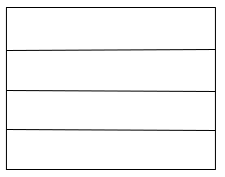
\includegraphics[width=0.29\textwidth]{1}}}
    \hspace{.1em}
    \subfigure{}\addtocounter{subfigure}{-2}
    \subfigure{\subfigure[条件方向的传统聚类]{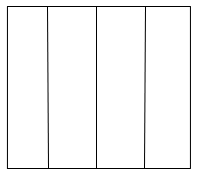
\includegraphics[width=0.25\textwidth]{2}}}
    \hspace{.1em}
    \subfigure{}\addtocounter{subfigure}{-2}
    \subfigure{\subfigure[双聚类]{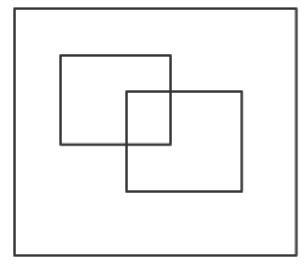
\includegraphics[width=0.25\textwidth]{3}}}
    \end{minipage}
    \vspace{0.2em}
    \caption{传统聚类与双聚类的区别}
    \label{fig:tradiAndBi}
    \end{figure}
    对于传统的聚类方法,其可以从基因或条件方向分别聚类,但是任一条件或基因都将被分配到某一类中去,这与现实中的情况是不符合的。而双聚类允许某些条件或基因不在任一类中出现。

\section{相关研究进展}
    从2000年双聚类分析被Cheng和Church引入到基因表达数据挖掘中到现在,双聚类分析经过了二十年的发展,许多优秀的算法被提出。由于双聚类分析是一个非常困难的问题,这一方向的研究一直在不断地进行着。殷路的研究将双聚类的发展过程大致分为了三个阶段。

    \subsection{早期阶段}
    该阶段的工作主要集中在模型和质量评价上。双聚类(Bicluster)这一单词最早由Hartigan于1972年提出,但Hartigan只是在行和列两个方向上分别聚类,没有全面地阐述双聚类的概念。直到2000年,Cheng和Church将双聚类引入到基因表达数据挖掘中,提出了CC算法,并得到了较好的效果。他们提出了MSR(Mean Square Residue,均方残差)用于评价双聚类相似性。MSR越小,则表明行相似性和列相似性越高。该算法先通过不断地删除基因节点和条件节点,找到小于事先给定的MSR阈值$\delta$的双聚类,然后将其作为初始双聚类,在保证MSR不会增大的前提下,不断向其中添加基因节点和条件节点,最终得到一个双聚类结果。如果想要多个结果,算法会把之前找到的双聚类使用随机数覆盖,再重复上述操作,直到获得想要数量的双聚类。随机数的引入,会导致结果不准确,而且无法找到重叠的双聚类。2002年,Yang等对CC算法进行改进,提出了FLOC算法。算法从多个初始双聚类出发,根据最大增益的原则,来执行基因和条件节点的删除或增加。但并没有解决贪心策略带来的陷入局部最优解的问题。

    Getz等提出了耦合双向聚类( Coupled Two-Way Clustering,CTWC)算法。 当CTWC应用于基因表达数据时,其目的是寻找基因的子集和条件的子集,从而单个细胞过程是条件子集上基因子集表达的主要贡献者。Busygin等提出了双共轭聚类算法(Double Conjugated Clustering,DCC),该算法在执行时,使用自组织映射(SOM)和角度度量(点积)来计算行和列之间的相似度。

    2002年,Bergmann 等人提出了ISA算法(Iterative Signature Algorithm,迭代签名算法)。ISA并没有使用MSR,而是将双聚类视为转录模块,然后通过对其进行打分,迭代地修改基因集和条件集,直到无法再继续修改。同年,Tanay等将双聚类定义为在条件(列)的子集之间存在连接反应(jointly respond )的基因(行)子集。 如果基因的表达水平相对于正常水平在该条件下发生显着变化,则该基因被认为对某种条件有反应,并提出了SAMBA(Statistical Algorithm Method For Bicluster Analysis)算法。该算法使用了图论和统计学的知识,将基因表达数据看作一个二分图,一边为基因,一边为条件。通过寻找最大稠密子图的方式来找到基因表达数据中的最大子矩阵,即双聚类。Lazzeroni 等把基因表达数据看作为背景模型与多个双聚类的叠加,并以此为基础提出了Plaid模型。Ben-dor等将双聚类建模为OPSM(Order Preserving Sub-Matrices),一个在基因表达水平上由连续保持的基因和条件组成的子矩阵,然后使用贪婪启发式算法在基因表达数据中搜索双聚类。出于同样的想法,Liu等将双聚类定义为OP-Clsuter(Order Preserving Cluster),算法的目标是找到在行方向具有变化趋势一致的双聚类。Murai等将双聚类建模为基因表达的保守模式xMotifs(Conserved Gene Expression Motifs),然后将随机选择的样本作为种子进行扩展,得到满足条件的双聚类,重复该过程,直到所有样本都包含在多个双聚类中。

    Segal等利用贝叶斯公式,在基因表达数据上结合先验信息建立了概率模型并称之为RPM (Rich Probabilistic Models)模型。该模型通过期望最大化 EM (Expectation Maximization)算法来确定双聚类。紧接着,Segal等又推广了RPM模型,使其能够允许双聚类出现重叠。Wang 等提出了pCluster指标来描述基因之间的相似距离,并将找到的双聚类为p-Cluster,然后通过枚举和减枝技术搜索基因表达数据中的双聚类。Sheng等基于Gibbs采样算法提出了一种双聚类分析算法。Gibbs采样避免了EM算法容易陷入局部最优的缺点,但是该算法在样本数量远小于基因数量时会有一定的计算困难。

    Califano等提出了一种算法,该算法解决了寻找有效$\delta$-valid模式的问题。他们的目标是找到在各列子集中表现出连贯值但在任何剩余的列中都没有任何连贯性的行组。在对数据进行预处理之后,他们使用模式发现算法来发现行和列候选集是具有统计意义的双聚类(其他候选集被丢弃)。最后,使用贪婪集覆盖算法从统计上重要的模式中选择最佳模式集,该算法将行和列添加到现有模式中,从而使它们成为最大模式。Kluger等通过假设归一化后的矩阵包含棋盘格结构,使用了一种频谱方法来进行双聚类分析。Tang等引入了相互关联的双向聚类(ITWC)算法,该算法结合了在数据矩阵的两个维度上进行单向聚类的结果,从而产生双聚类。 在对数据矩阵的行进行归一化之后,他们计算每行和预定义的稳定模式之间的矢量角度余弦值,以测试行值在列之间的变化是否很大,并删除变化不大的列。 之后,他们使用相关系数作为相似性度量来测量两行或两列之间的线性关系的强度,以执行双向聚类。

    \subsection{壮大阶段}
    该阶段相比早期阶段增加了在元启发式算法和多目标优化算法的研究。由于双聚类问题是NP难问题,通过贪婪或枚举的方法很难高效地得出结果,人们开始使用元启发式算法,如群智能算法来寻找双聚类。2004年,Bleuler等人设计了一个基因表达数据双聚类分析的进化算法框架。Chakraborty等同样基于进化算法提出了一种双聚类分析算法。不同于其他算法,该算法没有每一步都执行CC算法,而是只使用CC算法作为初始化步骤。初始种群包括通过K-均值聚类在基因和样本两个维度上结合生成的双聚类种子。紧接着使用进化算法按照适应值寻找容量大且更变化一致的双聚类。陈佳瑜结合量子粒子群和FLOC算法,将FLOC算法的输出作为量子粒子群的初始双聚类,取得了不错的效果。殷路提出了基于布谷鸟算法的双聚类算法,并与其他经典的群智能算法进行了比较。
    
    双聚类分析可以看作在均方残差,容量,方差等方向的多目标问题,许多算法使用多目标的方案解决双聚类问题。2006年Mitra提出了多目标进化双聚类的框架,应用经典的非支配排序遗传算法( Non-dominated Sorting Genetic Algorithm-II,NSGA-II)算法,整合局部搜索策略,并提出新的定量度量方法估计双聚类的质量。2007年,Divina 等提出多目标连续变化双聚类算法 (Sequential Multi objective Biclustering,SMOB)。Coelho等提出了一种基于多目标人工免疫系统的双聚类技术,它能够执行多种群搜索,名为MOM-aiNet。Giraldez应用最大标准区域(Maximal Standard Area,MSA)作为度量双聚类的标准,并和MSR一起应用到多目标进化算法MOEA中,有效解决了成比例模式的双聚类问题。2013 年Brizula等提出了一种改进的多目标遗传双聚类算法(Enhanced Multi-objective Genetic Biclustering ,EMOGB)。    

    一些双聚类算法在开发双聚类算法中采用模糊集理论来捕获重叠的双聚类。Tjhi等提出了一种灵活的模糊双聚类算法,该算法称为具有特征聚类加权的灵活模糊联合聚类(Flexible Fuzzy Co-clustering with Feature-cluster Weighting,FFCFW),算法将特征聚类加权纳入了公式,允许对象聚类的数量与特征聚类的数量不同。对于由FFCFW生成的每个目标聚类,都采用了一个特征聚类权重方案,以便在特征聚类权重中体现两种类型的聚类之间的关系。这使FFCFW可以更准确地表示模糊共聚体。另外,FFCFW使用迭代的思想进行优化。2007年,Fei X等提出了一种基于遗传算法的模糊双聚类算法GFBA。该算法没有使用二进制串来表示双聚类,而是通过0到1之间的实数值代表相应基因和条件在该双聚类中参与程度。2008年,Han L等提出了FBMDA(Fuzzy Biclustering for Microarray Data Analysis)算法。该方法结合了Nelder-Mead算法和min-max算法来构造分层结构的双聚类,因此可以表示不同级别的双聚类信息。FBMDA使用多目标优化,可同时优化容量,方差和模糊熵。Nelder-Mead算法用于计算单个目标最优解,而min-max算法用于在多个目标之间进行权衡。

    基于图理论的双聚类在这一阶段也得到了发展。Prelic等提出了BiMax(Binary inclusion-Maximal)双聚类算法。算法首先根据用户指定的阈值将输入矩阵离散为0和1,基于此二进制矩阵,BiMax可以识别所有最大的双聚类,其中双据类被定义为包含所有1的子矩阵E。inclusion-Maximal表示此双聚类没有完全包含在任何其他双聚类中。基于矩阵E可以推算出双聚类的事实,算法使用增量算法来搜索inclusion-maximal双聚类。由于BiMax与二进制矩阵一起使用,因此它仅适用于检测恒定值的双聚类。2007年,Ahmad等将双聚类分析问题转化为加权二部图中最大交叉数减少(最小化)问题,并提出了一种称为cHawk的算法。该算法采用了重心启发式和局部搜索技术。首先,从输入矩阵中构建二分图,然后进行二分图交叉最小化,最终确定双聚类。此方法对矩阵进行重新排序,以使属于同一个双聚类的所有行和列都靠的更近。cHawk能够检测恒定值以及加法模型和重叠的双聚类。

    
    \subsection{当前阶段}
    随着大数据,集成学习,深度学习等技术的发展和普及,许多新型的双聚类分析算法涌现出来。当前阶段除了元启发式算法,双聚类模型和质量评价指标和多目标优化算法之外,增加了以这些新型技术为基础的双聚类研究。基于 Bayesian 理论和双聚类的 Plaid 模型, Zhang 等提出了 Bayesian Plaid模型。Liu 等提出了基于GPU的统一计算设备体系结构(CUDA)的并行 GBC 算法。另外,集成学习因其在聚类方向的广泛应用,也被引入到双聚类分析中。Hanczar 等应用bagging技术提高CC和Plaid算法的结果质量。基于谱技术,Huang 等提出了SCCE(Spectral Co-Clustering Ensemble)双聚类算法。近年来的研究使得神经网络这种深度学习技术取得了突飞猛进的发展,其强大的能力不断地让人们感到惊叹。Sun 等基于深度学习技术提出了自动解码机(AutoDecoder)算法用来寻找双聚类。

    该阶段有关模式挖掘和关联分析出现了不少的研究工作。Yoshifumi等提出了BiModule算法,该算法允许对输入矩阵进行参数化的多值逐项列出,以使用LCM挖掘算法发现从(闭合)频繁模式中得出的常数双聚类。DeBi从使用MAFIA挖掘算法在二值化矩阵上挖掘的(最大)频繁模式中获得双聚类,并放置关键的后处理原理对其进行调整,以确保其统计意义。Rui Henriques等提出的BicPAM通过对输入矩阵执行迭代校正,扩展了先前方法的恒定假设,以找到具有对称,加法和乘法因子的双聚类。BicPAM还引入了为单个元素分配多个离散值的可能性,从而克服了离散化问题,并提供了新的策略来稳健地处理噪声和缺失值。Bellay等使用Apriori算法与其他原理结合使用,以评估所发现的双聚类相对于背景噪声的功能一致性。 Martinez等提出了GenMiner算法,该算法在输入矩阵中包括外部知识边缘,以从关联规则中导出双聚类,该关联规则将注释(行或列的外部分组)与使用CLOSE关联规则算法从(闭合)频繁模式得出的聚类相关联。BiP算法由Henriques等提出,通过依靠耐噪声的关联规则来发现plaid模型,以恢复表观噪声区域,这是由于在双聚类之间重叠区域上存在累积效应。

    2013年,Yan提出了可以根据不同双聚类类型执行不同搜索策略的RGCE-B(Biclustering based on Related Genes and Conditions Extraction)算法。他们根据基因以及条件的稳定性和不同的双聚类类型将层次聚类应用于从输入数据生成的不同数据矩阵。另外,作为预处理步骤,使用James–Stein方法和内核估计原理估计丢失的数据,其中k均值用于获取估计矩阵。Hussain等利用明可夫斯基距离和层次聚类提出了SBB(Similarity Based Biclustering)算法。

    2014年,Ahmed等最近提出了一种基于双聚类的移动和缩放相关性(Shifting and Scaling Similarity,SSSim)来评估双聚类的相似性度量,并基于此度量提出了ICS(Intensive Correlation Search)算法。SSSim是使用基线(参考)条件对以及其他条件对的基因局部方法定义的。当评估基因对时,所得分数为从0到1不等,其中值为1表示两个基因都表现出完美的移位和缩放相关性。为了评估双聚类,使用两个输入参数$\tau$和$\alpha$分别考虑基因与部分或完整双聚类之间的相关性。ICS策略迭代地提取不同对基因的相关子空间。这些相关的子空间对应于最大样本集,对于这些样本,基因表达的相关性超过了用户定义的阈值$\tau$。子空间对应于双聚类,该双聚类最初由一对基因形成,并且也被迭代扩展以包括更多基因,直到不能再向双聚类添加任何基因为止。该扩展阶段由第二用户定义的阈值$\alpha$控制。形成初始相关子空间的初始基因对必须由迄今为止不在任何已产生的双聚类的基因形成。但是,这种限制并不能阻止基因在延伸阶段成为多个双聚类的一部分,从而允许双聚类之间的重叠。

    2015年,Chekouo等提出了PPM模型(Penalized Plaid Model),该模型主要关注的是阐明双聚类算法背后的相关统计模型。他们发现,许多已知的技术都有潜在的贝叶斯隐患。这一特征促使他们采用贝叶斯框架对双聚类进行建模,并在先前的工作中纳入了两个主要特征:选择双聚类数量的标准和用于解决双聚类之间重叠的惩罚性朴素模型。在此模型中,由于双聚类模型中参数的数量随双聚类的数量呈指数增长,因此采用hard-EM算法用于参数估计。

    基于共享相似途径的两个基因可能相似的假设,Mandal等提出了POPBic(Pathway-based Order Preserving Biclustering)算法。POPBic方法的基本原理是在具有大量共同途径的一对基因之间应用最长共同子序列的概念。Singh提出了一种基于图的可调谐双聚类算法(TuBA),该算法基于一种新颖的成对接近度度量,该度量利用数据集的大小来识别肿瘤样本的子集,这些子集相对于其他样本基因以其最高或最低水平共表达。


\section{论文主要工作}
    因为基因表达数据上双聚类分析的困难性和重要性,过去提出的大量算法都有各自的侧重点。有关基于元启发式的双聚类分析算法,缺少一个较为完整的完整的分析工作。本文以提高双聚类结果的质量指标和生物意义为目标,结合混合元启发式方法和多目标优化方法,对双聚类分析这一问题进行了综合比较研究。本文主要工作如下:
    \begin{itemize}
       \item[1.] {考虑到布谷鸟搜索算法和萤火虫算法的优势互补,本文提出了一种基于布谷鸟搜索和萤火虫算法的混合双聚类分析算法(Cuckoo Search and Firfly Algorithm hybrid Biclustering,CSFAB)。首先,将均方残差,基因容量和样本容量的权重之和作为适应值函数。然后将连续的解转换成比特串来表示双聚类,经过几种混合方式的比较之后,选择了最佳的混合方案。最后在四个常用且数据规模大小不一的基因表达数据集上,通过实验对算法的有效性进行了分析和验证。}

       \item[2.] {双聚类分析其实是多目标优化问题。本文提出了一种多目标细菌觅食算法的双聚类分析算法(Multi-object Bacterial Foraging Algorithm Biclustering,MOBFOB)。算法将均方残差,基因容量和样本容量看作待优化指标,并按照被支配次数对种群排序。以细菌觅食算法为指导,不断地寻找占优的双聚类,并将其保存在外部集合中。最后在四个基因表达数据集上,通过实验对算法的有效性进行了验证。}
       
    \end{itemize}

\section{论文组织结构}
    本文首先对基因表达数据和双聚类分析等相关基础知识进行阐述。然后从单目标优化,混合优化和多目标优化等方面,研究了以群智能算法如布谷鸟搜索算法、萤火虫算法和细菌觅食算法为框架的双聚类算法。最后对本文的工作进行了总结和展望。全文共有五章,本文各章节内容安排如下:

    第一章从生物背景知识出发,讨论了基因研究的重要性以及双聚类的作用和发展现状。双聚类克服了常规聚类与基因表达数据之间的矛盾,能更好的挖掘出有价值的基因子集和条件子集。群智能算法由于其快速且效果更好,在双聚类分析中得到了很广泛地应用。

    第二章先是更具体地讨论的基因表达数据的数学形式,以及双聚类的定义、类型和结构。接着将双聚类算法分为了基于质量评价指标和基于模型两种。然后,对于双聚类结果,讨论了其质量验证指标和生物验证指标。最后分别介绍了本文所关注的群智能算法。

    第三章为了解决普通双聚类算法的质量评价指标不足和生物意义不明显的缺点,本文将布谷鸟算法与萤火虫算法进行了融合,并提出了CSFAB双聚类算法。通过实验,确定了融合的最佳方案,并从质量评价指标和生物评价指标的角度进行了比较分析。

    第四章首先介绍了多目标优化的基本概念,接着将细菌觅食算法按照多目标优化和双聚类的特点进行了改进,包括适应值函数,以及互不支配时的比较规则,并提出了MOBFOB算法。最后根据适应值曲线和生物指标对算法进行了分析。
    
    第五章对全文工作进行了总结和展望。


% !Mode:: "TeX:UTF-8"
\chapter{基因表达数据的双聚类相关概述}

\section{基因表达数据}
  数据的好坏在很大程度上决定了结果的上限,而算法只是去逼近这个上限,因此了解数据本身是很有必要的。基因表达数据主要通过基因芯片技术和下一代测序技术等这些高通量基因表达测量技术获得。这些技术可以同时在不同的样本或条件下,对成千上万的基因进行高效、精确、定量地测量。大致的流程为,制备芯片、制备样本、标记和杂交、洗涤和绘制图像,获取结构化数据。首先,准备一个具有成千上万个网格的微阵列芯片,该芯片的每个网格里面都放置着一个DNA探针。接着准备两条mRNA,一条用于测试,另一条作为控制样本。对这两条mRNA进行逆转录,得到互补脱氧核糖核酸(cDNA),并使用荧光染料或放射性同位素对cDNA进行标记。将标记后的cDNA与微阵列芯片中的DNA进行杂交,然后清洗掉多余的杂交液。最后,通过芯片扫描仪获得芯片在杂交后各个DNA探针的荧光染料或放射性同位素强度,并绘制成信号强度图。通过专业的软件将图像转化为结构化的数字信息,得到基因表达数据。
  
  这时只是得到了一些原始数据,由于在特定条件下只有很少数的基因会表达,里面会存在很多缺失数据和噪声。需要对原始数据进行缺失值和去噪处理,才能得到适合数据挖掘的数据。一般来说,有两种方法处理缺失值:一是直接丢弃存在缺失值的行和列;二是根据已知的数据对缺失值进行填充,该种方法有可能会对原始数据产生不利的影响,改变真实数据的分布,需要根据数据特点选择不同的填充策略。

  基因表达数据一般以一个二维矩阵\textit{E}表示,一行代表一个基因,一列代表一个实验条件。实验条件包括不同时期,不同组织,不同个体,不同外部环境等等。矩阵\textit{E}中的每个元素$e_{ij} $表示基因$g_i$在实验条件$c_j$下的表达水平值,其生物含义是该基因在此条件下,细胞中mRNA的含量。矩阵\textit{E}中的每一行被称为基因在该基因表达数据上的全局表达模式(Expression Pattern)。矩阵\textit{E}中的每一列被称为条件在该基因表达数据上的全局表达描述(Expression Profile)。

  基因表达数据极其庞大,以及需要非常专业的生物学知识,导致很多跨领域的研究者很难涉足。为了打破这种学科壁垒,科学家们提出了关于描述和存储基因表达数据的标准,如序列、平台和数据集,并在标准之上建立了基因表达数据库。最广泛的数据库为GEO(Gene Expression Omnibus),由美国国家生物技术信息中心于2000年开发。该数据库提供了共享基因表达数据的平台,并且有专业的人员进行审核。公共数据库的出现,极大促进了生物信息学的发展。
\section{双聚类的相关概念}

  \subsection{双聚类的定义}
  给定一个大小为$n\times m$基因表达数据$\textit{E(X,Y)}$,假定集合$I\subseteq X,(|I| = k \leq n)$是\textit{E}的基因集合$X$的子集;集合$J\subseteq Y,(|J| = l \leq m)$是\textit{E}的基因集合$Y$的子集。如图\ref{fig:define_bic}所示,双聚类是指在条件子集$J$下的基因表达模型表现出同源特性的基因子集$I$。因此,双聚类可以定义为一个$k \times l$的子矩阵$B(I, J)$,也简称为$B$。
  \begin{figure}[htbp]
      \centering
  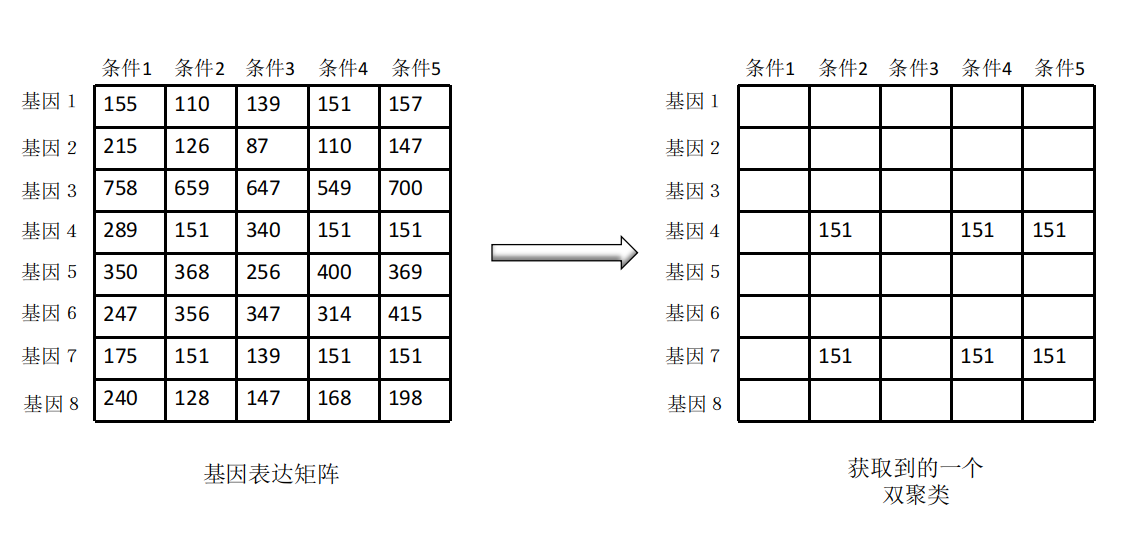
\includegraphics[width = 0.8\textwidth]{aBicluster.png}
  \caption{双聚类定义示例}
  \label{fig:define_bic}
  \end{figure}

  \subsection{双聚类的类型}
  给定一个二维矩阵$A(I,J)$,$a_{ij}$为其中第$i$行第$j$列的值,$\alpha_i$是一个与行有关而与列无关的变量,$\beta_j$是一个与列有关而与行无关的变量,$0\le h,r,t,d \le |I|$或$0\le h,r,t,d \le |J|$。Madeira 和 Oliveira提出,在双聚类中主要有以下四种类型:
  \begin{enumerate}
    \item[1.] 具有相同常量值的双聚类。该类型的双聚类所有的元素为同一个常量,如图\ref{bic61}所示,公式如下。
    \begin{equation}
      a_{ij}=\mu
    \end{equation}

    \item[2.] 列或行具有相同常量值的双聚类,满足公式\ref{equ:hang}的双聚类属于行常量值双聚类,如图\ref{bic62}所示。满足公式\ref{equ:lie}的双聚类属于列常量值双聚类,如图\ref{bic63}所示。
    \begin{equation}\label{equ:hang}
    a_{ij}=\mu+\alpha_i \mbox{或} a_{ij}=\mu *\alpha_i 
    \end{equation}
    \begin{equation}\label{equ:lie}
    a_{ij}=\mu+\beta_j  \mbox{或} a_{ij}=\mu *\beta_j
    \end{equation}
    
    \item[3.] 数值一致的双聚类,如图\ref{bic64}和\ref{bic65}所示,满足的公式如下。
    \begin{align}
    a_{ij}=\mu+\alpha_i+\beta_j \label{equ:jiafa}\\
    a_{ij}=\mu *\alpha_i*\beta_j\label{equ:chengfa}
    \end{align} 

    \item[4.] 具有连贯演变的双聚类,如图\ref{bic66}所示,公式如下。
    \begin{align}
    a_{ih}\le a_{ir}\le a_{it}\le a_{id} \\
    a_{hj}\le a_{rj}\le a_{tj}\le  a_{dj} 
    \end{align}
  \end{enumerate}

  \begin{figure}[htbp]
  \setlength{\subfigcapskip}{-1bp}
  \centering
  \begin{minipage}{.7\textwidth}
  \centering
  \subfigure{\label{bic61}}\addtocounter{subfigure}{-2}
  \subfigure{\subfigure[]{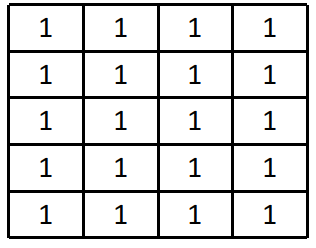
\includegraphics[width=0.3\textwidth]{a-bic}}}
  \hspace{.2em}
  \subfigure{\label{bic62}}\addtocounter{subfigure}{-2}
  \subfigure{\subfigure[]{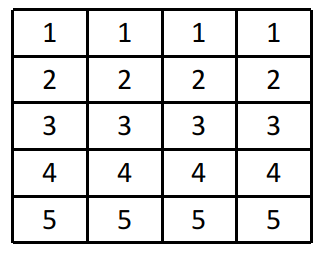
\includegraphics[width=0.3\textwidth]{b-bic}}}
  \hspace{.2em}
  \subfigure{\label{bic63}}\addtocounter{subfigure}{-2}
  \subfigure{\subfigure[]{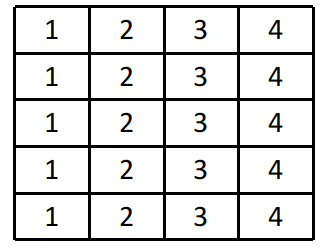
\includegraphics[width=0.3\textwidth]{c-bic}}}
  \end{minipage}
  \centering
  \begin{minipage}{.7\textwidth}
  \centering
  \subfigure{\label{bic64}}\addtocounter{subfigure}{-2}
  \subfigure{\subfigure[]{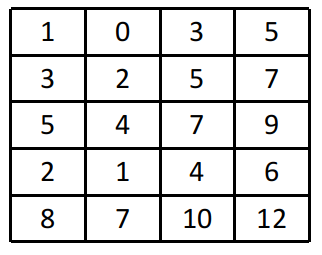
\includegraphics[width=0.3\textwidth]{d-bic}}}
  \hspace{.2em}
  \subfigure{\label{bic65}}\addtocounter{subfigure}{-2}
  \subfigure{\subfigure[]{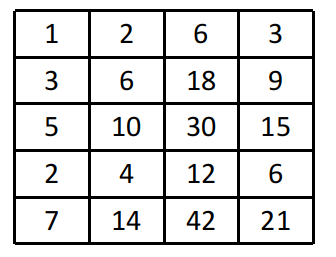
\includegraphics[width=0.31\textwidth]{e-bic}}}
  \hspace{.2em}
  \subfigure{\label{bic66}}\addtocounter{subfigure}{-2}
  \subfigure{\subfigure[]{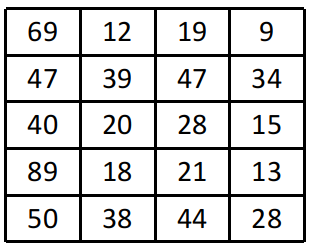
\includegraphics[width=0.3\textwidth]{f-bic}}}
  \end{minipage}
  \vspace{0.2em}
  \caption{双聚类的类型}
  \end{figure}

  \subsection{双聚类的结构}
  双聚类的结构是指,通过算法找到的双聚类之间在原始矩阵时间的相对位置。根据结构,大体可以分为8类:
  \begin{figure}[!h]
  \setlength{\subfigcapskip}{-1bp}
  \centering
  \begin{minipage}{.8\textwidth}
  \centering
  \subfigure{\label{bic81}}\addtocounter{subfigure}{-2}
  \subfigure{\subfigure[单一结构]{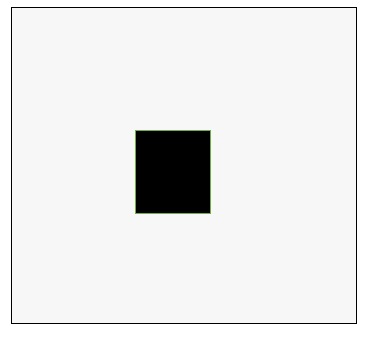
\includegraphics[width=0.2\textwidth]{struct1}}}
  \hspace{.2em}
  \subfigure{\label{bic82}}\addtocounter{subfigure}{-2}
  \subfigure{\subfigure[对角结构]{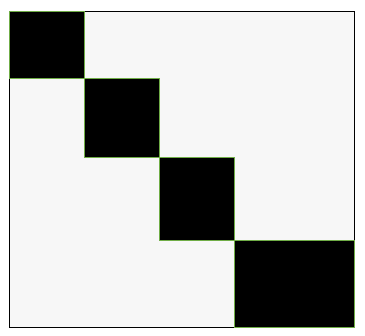
\includegraphics[width=0.2\textwidth]{struct2}}}
  \hspace{.2em}
  \subfigure{\label{bic83}}\addtocounter{subfigure}{-2}
  \subfigure{\subfigure[棋盘结构]{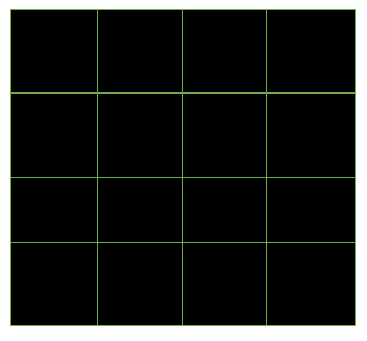
\includegraphics[width=0.2\textwidth]{struct3}}}
  \hspace{.2em}
  \subfigure{\label{bic84}}\addtocounter{subfigure}{-2}
  \subfigure{\subfigure[行互斥结构]{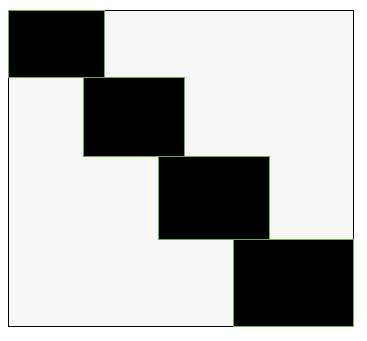
\includegraphics[width=0.2\textwidth]{struct4}}}
  \end{minipage}
  \centering
  \begin{minipage}{.8\textwidth}
  \centering
  \hspace{.2em}
  \subfigure{\label{bic85}}\addtocounter{subfigure}{-2}
  \subfigure{\subfigure[列互斥结构]{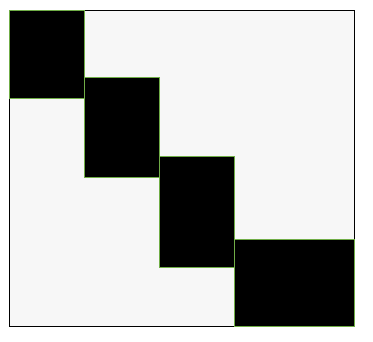
\includegraphics[width=0.2\textwidth]{struct5}}}
  \hspace{.2em}
  \subfigure{\label{bic86}}\addtocounter{subfigure}{-2}
  \subfigure{\subfigure[非互斥且非重叠结构]{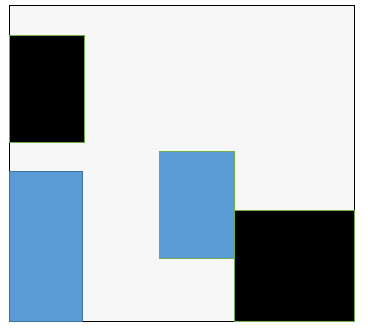
\includegraphics[width=0.2\textwidth]{struct6}}}
  \hspace{.2em}
  \subfigure{\label{bic87}}\addtocounter{subfigure}{-2}
  \subfigure{\subfigure[嵌套重叠结构]{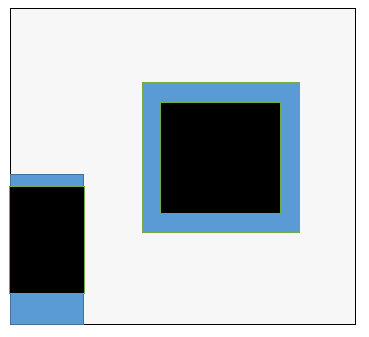
\includegraphics[width=0.2\textwidth]{struct7}}}
  \hspace{.2em}
  \subfigure{\label{bic88}}\addtocounter{subfigure}{-2}
  \subfigure{\subfigure[任意重叠结构]{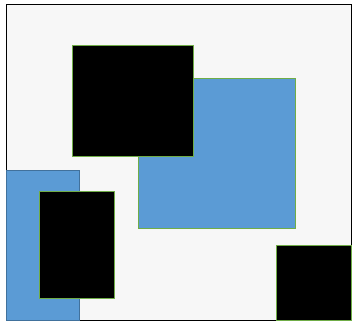
\includegraphics[width=0.2\textwidth]{struct8}}}
  \end{minipage}
  \vspace{0.2em}
  \caption{双聚类的结构}
  \label{fig:bic-struct}
  \end{figure}
  \begin{enumerate}
    \item[1.] 单一结构。指基因表达数据中只存在一个双聚类,且基因和条件可以不属于该双聚类,如图\ref{bic81}所示。
    \item[2.] 对角结构。指任意两个双聚类之间互不共享行和列,且任一行或列只能属于其中一个双聚类,如图\ref{bic82}所示。这类的双聚类可以通过交换位置,最后呈对角线形状。
    \item[3.] 棋盘结构,指通过传统的聚类方法分别对行和列进行聚类,然后组合得到的双聚类,如图\ref{bic83}所示。
    \item[4.] 行互斥结构。指双聚类之间不存在共享的行,可以看作有对角线结构放松对行的限制所得,如图\ref{bic84}所示。
    \item[5.] 列互斥结构。与行互斥相似,指双聚类之间不存在共享的列,如图\ref{bic85}所示。
    \item[6.] 非互斥且非重叠结构。之允许双聚类之间存在相同的行或列,但不能存在重叠和包含关系,如图\ref{bic86}所示。
    \item[7.] 嵌套重叠结构。指双聚类之间可以存在包含关系,但不能出现重叠关系,如图\ref{bic87}所示。
    \item[8.] 任意重叠结构。指双聚类之间即可以存在包含关系,也可以存在重叠关系,如图\ref{bic88}所示。
  \end{enumerate}

  传统的聚类只能找到像图\ref{bic81}所示的单一结构,这对于基因表达数据的挖掘是远远不够的。嵌套和重叠的结构要比非嵌套和非重叠的结构复杂,需要更复杂的算法来找到它们。

  
\section{双聚类的评价指标}
  \subsection{质量评价指标}\label{section:qualityEval}
  由于在基因表达数据进行双聚类分析是NP难问题,目前大部分的算法都是基于优化策略的。为了评价双聚类的质量和知道优化的方向,需要有效的评价指标。指标是否科学可靠直接会体现到双聚类结果上。本节对目前常用的评价指标进行一个总结。
  
  方便起见,先引入一些数学定义。给定一个大小为$n\times m$的基因表达数据$E(X,Y)$,以及一个大小为$k\times l$的双聚类$B(I,J)$,$b_{Ij}$为$B$中第$j$列的平均值,$b_{iJ}$为$B$中第$i$行的平均值,$b_{IJ}$为双聚类整体的平均值,$Vol_B$表示双聚类的体积,公式定义如下:
  \begin{align}
    b_{iJ} &= \sum_{j\in J}\frac{b_{ij}}{|J|} \\
    b_{Ij} &= \sum_{i\in I}\frac{b_{ij}}{|I|} \\
    b_{IJ} &= \sum_{i\in I,j\in I}\frac{ b_{ij} }{|I| \times |J|}\\
    Vol_B &= |I| \times |J|
  \end{align}
  \begin{enumerate}
    \item[1.] 方差。用$Var(B)$表示双聚类$B(I,J)$的方差,该指标代表了该双聚类的变化幅度,越大则双聚类中的值越不相同,定义如下:
    \begin{equation}
      Var(B) = \sum_{i\in I,j\in I}\frac{(b_{ij}-b_{IJ})^2}{Vol_B}
    \end{equation}

    \item[2.] 均方残差。该指标首先在CC算法中提出,并被广泛地应用在基因表达矩阵的分析中。数学定义如公式\ref{equ:msr}所示。该指标适合寻找像式\ref{equ:jiafa}这样的加法模型双聚类,且值越小越符合该模型。
    \begin{equation}\label{equ:msr}
      MSR(B) = \frac{1}{Vol_B}\sum_{i=1}^k\sum_{j=1}^l(b_{ij}-b_{iJ}-b_{Ij}+b_{IJ})^2
    \end{equation}

    \item[3.] 扩展均方残差。因为$MSR(B)$只能发现加法模型,Mukhopadhyay 等提出了扩展均方残差(Scaling Mean Squared Residue,SMSR)。该指标适合寻找如\ref{equ:chengfa}这类的乘法模型双聚类,且值越小越符合该模型。双聚类$B(I,J)$的SMSR(B)定义如下:
    \begin{equation}\label{equ:smsr}
      SMSR(B) = \frac{1}{Vol_B}\sum_{i=1}^k\sum_{j=1}^l(\frac{b_{iJ}\times b_{Ij}-b_{ij}\times b_{IJ}}{b_{iJ}\times b_{Ij}})^2
    \end{equation}

    \item[4.] 相关指数。该指标用来寻找列值常量类型的双聚类,定义如下:
    \begin{equation}
      RI(B) = \sum_{j=1}^l R_{Ij}/l = \sum_{j=1}(1 - \frac{\sigma_{Ij}^2}{\sigma_j^2})/l
    \end{equation}
    \hspace{2em} 其中,$R_{Ij}$为双聚类中第$j$列的相关指数,$\sigma_{Ij}^2$是双聚类中第$j$列所有元素的局部方差,$\sigma_{j}^2$是基因表达数据第$j$列所有元素的全局方差。该指标越大则越符合列值常量类型。类似的,稍加改造则可以寻找行值常量类型的双聚类。

    \item[5.] 最大标准化区域。该指标由Giraldez 等提出,并用于寻找趋势一致的双聚类。计算过程:首先要对双聚类$B(I,J)$进行标准化,得到$\hat{B}(I,J)$,计算公式为:
    \begin{equation}
      \hat{b}_{ij} = \frac{b_{ij}-b_{iJ}}{\sigma_i}
    \end{equation}
    \hspace{2em} 其中,$b_{iJ}$和$\sigma_i$为双聚类$B$中第$i$行元素的平均值和标准差。根据$\hat{B}(I,J)$,双聚类$B(I,J)$的最大标准化区域的定义如下:
    \begin{equation}
      MSA(B) = \sum_{j=1}^l \mid \frac{M_j-m_j-M_{j+1}+m_{j+1}}{2}\mid
    \end{equation}
    \hspace{2em} 其中,$M_j=max_{i\in [i,k]}\hat{b}_{ij}$,$m_j=min_{i\in [i,k]}\hat{b}_{ij}$。当双聚类中基因表达模型完全一致时,$MSA(B)=0$。

    \item[6.] HV-Score。一个双聚类$B(I, J)$的Hv-Score定义如下:
    \begin{equation}
     Hv(B) = \frac{\sum_{i=1}^k \sum_{j=1}^l(b_{ij}-b_{iJ}-b_{Ij}+b_{IJ})^2}{\sum_{i=1}^k \sum_{j=1}^l(b_{ij}-b_{iJ})^2}
    \end{equation}
    该指标是对MSR的改进,改善了MSR偏向找到常量类型双聚类的不足,由Bryan等提出。值越小则双聚类的质量越好。

    \item[7.] 覆盖率。该指标是双聚类集合的多样性指标,因为大多数算法找到的双聚类都不止一个,如果双聚类过度重合则意义不大。我们总是希望找到互相重叠小且能覆盖到更多的基因表达数据的双聚类集合。 假设双聚类集合$\Pi=\{B_1,B_2,...,B_r\}$,$\phi_k(E)$为判断$E(X,Y)$中每个元素$e_{ij}$是否在双聚类$B_k$的函数。定义公式如下:
    \begin{equation}
    \phi_k(a_{ij})  = \left\{
      \begin{aligned}
       1 & = & if a_{ij} \in B_k \\
       0 & = & otherwise 
      \end{aligned}
    \right.
    \end{equation}
  \end{enumerate}
  \hspace{2em}则双聚类集合$\Pi$的覆盖率$covRate(\Pi)$定义如下:
  \begin{equation}
   covRate(\Pi) = \frac{\sum_{i=1}^k\sum_{j=1}^l\cup_{k=1}^r\phi_k(a_i)}{n \times m} 
  \end{equation}
  \hspace{2em}从定义可以看出,覆盖率的含义是集合$\Pi$中$r$个子矩阵并集所占基因表达数据$E$的比例。

  \subsection{生物评价指标}
  为了评价通过双聚类获得基因集合的生物意义,需要对其进行基因解释。生物技术的发展积累了很多关于基因的描述,这些信息可以为我们提供参考。目前,最流行的基因注释数据库当属KEGG数据库和GO数据库。前者主要用来做旁路分析,所谓旁路分析,就是获得基因之间的调控关系,后者主要用来做富集分析,对基因功能进行注释。目前对双聚类结果的生物验证主要还是GO的富集分析。

  GO数据库中保存了各种物种的基因的注释信息,包括基因的功能和之间的关系。GO将基因的功能分为分子功能(Molecular Funciotn,MF),细胞组成(Cell Compose,CC)和生物过程(Biological Process,BP)。GO将一项功能称为一个GO项(term),并通过一个有向无环图表示项与项之间的关系。如果两个GO项之间有连线,则表示之间存在联系。如果双聚类中关于某一GO项的基因个数大于该项随机概率出现的次数,则称该双聚类的基因集合富集在这一GO项,并用通过统计学方法,得到统计值P-value来表示富集的程度。P-value越小,则富集程度越大,一般只关注P-value小于0.01的GO项。  
  \begin{enumerate}
    \item[1.] 显著富集双聚类的比例。对于双聚类集合$\Pi=\{B_1,B_2,...,B_r\}$,假设其中存在$r_{sig} \le r$个双聚类存在富集。显著富集双聚类的比例(Proportion of the biclustersSignificantly Enriched, proSigEnriched)定义如下:
    \begin{equation}
      proSigEnriched = \frac{r_{sig}}{r} \times 100\%
    \end{equation}

    \item[2.] 带权重的富集分数。$proSigEnriched$只是在双聚类层面的验证指标,不仅没有精确到功能项而且对于基因集合很大的双聚类很难区分。所以,带权重的富集分数(Weight Enrichment Score, WEScore)被引入进来,定义如下:
    \begin{equation}\label{equ:wescore}
      WEScore = \sum_{i=1}^t{x_i s_i}/k
    \end{equation}
    \hspace{2em}其中,$t$是双聚类$B$经过GO分析后得到的GO项的个数,$x_i$是对应第$i$个GO项的基因个数,$s_i$是对应GO项经过负对数变换后的P值,$k$是双聚类中基因的个数。$WEScore(B)$越大则该双聚类生物意义越大。

    \item[3.] 平均P值。与$WEScore$类似,平均P值(Mean of P Values, meanPValue)的定义如下:
    \begin{equation}\label{equ:meanP}
      meanPValue = \sum_{i=1}^ts_i/t
    \end{equation}
    \hspace{2em}其中,$t$与$s_i$与公式\ref{equ:wescore}含义一样,且$meanPValue(B)$越大则该双聚类生物意义越大。

    \item[4.] 基因与GO项的比值。由于一个双聚类一般会在很多个GO项出现富集,如果GO项的个数越少,则说明双聚类中的基因之间越相关。因此,引入了基因与GO项的比值(Ratio of number of gene to number of significant terms, rateGeneTerm),定义如下:
    \begin{equation}
     rateGeneTerm(B) = k / t 
    \end{equation}
    \hspace{2em}其中,$k$和$t$与公式\ref{equ:wescore}中含义一致。
  \end{enumerate}

\section{双聚类算法的分类}
为了解决双聚类这一难题,大量的算法被提出。有的算法使用质量评价指标来指引着双聚类搜索过程,有的则使用其他策略解决问题。基于此,本文将双聚类分析算法大致分为基于质量评价的双聚类算法和基于模型的双聚类算法。

  \subsection{基于质量评价的双聚类算法}
  因为在基因表达数据上进行双聚类分析是NP难问题,所以无法通过穷举的方式来搜索双聚类。上一节给出了一些质量评价指标,大部分算法都是使用不同的策略,找到在一种或多种评价指标最优的双聚类。根据搜索策略的不同,可以将算法分为以下几类。
  \begin{enumerate}
    \item[1.] 基于贪婪迭代搜索策略。这类算法,一般是从一个初始的双聚类出发,然后根据质量指标迭代地添加或移除基因或条件节点。该类算法的有点是速度快,但通常质量欠佳。MSB(Maximum Similarity Biclusters)算法以及CC算法就其中的典型算法。

    \item[2.] 基于随机贪婪搜索。跟前一种不同的是,此类算法在迭代过程中并不只考虑最优的操作,而是一定概率采取次优的操作,保证了搜索的多样性。FLOC算法就属于此类。
    
    \item[3.] 基于聚类算法。该类算法的特点是,先使用传统的聚类方法分别对行和列进行聚类,并将其组合起来,然后在组合得到的双聚类中挑取质量评价较好的结果。例如,PSB算法先使用IPC聚类算法在行和列两个方向聚类分析,然后使用MSR(B)筛选组合后得到的双聚类。
    
    \item[4.] 基于元启发式算法。元启发算法的特点是模拟大自然中生物的高效的搜索行为,例如例子群算法,蚁群算法。这类算法通过使用双聚类的质量评价指标组合成适应度函数,从而找到质量评价指标高的双聚类。
  \end{enumerate}

  \subsection{基于模型的双聚类算法}
  在有些双聚类分析算法中,并没有使用质量评价指标,该类算法被称为基于模型的双聚类算法。根据算法使用的数学模型或结构的不同,将这些算法分为以下几类:
  \begin{enumerate}
    \item[1.]基于图论的双聚类分析方法。计算机科学中的图可以用二维矩阵表示,将图论中的知识迁移到基因表达数据的双聚类分析中,是该类算法的显著特点。例如,SAMBA 和 Bi-Force 算法将基因表达数据转换为带权重的二分图,双聚类则被视为其中的二分团(biclique)。MicroCluster 算法将基因表达数据转换为带权有向多重图,双聚类分子转化为深度搜索树。

    \item[2.]基于概率模型的双聚类分析方法。概率论和数理统计在挖掘海量数据方面有着强大的理论支持。这类方法通过在基因表达数据上建立统计模型,通过优化模型参数来找到优质的双聚类。这类算法有,基于 Gibbs采样理论的 QDB 算法以及对 Plaid 模型改进的 PPM 算法。
    
    \item[3.]基于矩阵论的双聚类分析方法。基于矩阵论和线性代数,通过线性变换和矩阵分解等理论来寻找双聚类是这类算法的主要手段。比如,ISA算法中就间接用到了奇异值分解(SVD)。nsNMF算法使用非负矩阵分解(NMF)来寻找双聚类。
    
    \item[4.]基于关联规则挖掘的双聚类分析方法。将在业务数据上发现最大频繁项的问题,与在基因表达数据中双聚类分析问题联系起来,是该类算法的主要特点。基于关联规则的挖掘算法在商业上有着广泛地应用,通过类比的思想,这类的双聚类分析算法取得了不错的效果。具有代表性的算法有BiModule算法和Fdcluster算法。
    
  \end{enumerate}

\section{群智能算法}
目前,有很多优秀的优化算法,有确定性方法如线性规划、二次规划,动态规划和梯度下降;以及随机性方法如群体智能。这些方法帮助我们能够在一定的时间内解决某些问题。然而,处理大量高维数据时,确定性方法太过复杂导致需要大量的计算成本。元启发式的群体智能算法因其高效率越来越受到关注。

  \subsection{粒子群算法}
  粒子群(Particle Swarm Optimization,PSO)算法是Kennedy和Eberhart于1995年提出的一种群体智能优化算法,其流程图如图\ref{fig:pso}所示。该算法是受到了鸟群觅食过程中的集体行为的启发。PSO 算法将群体中的粒子看作可行域中的一个点,这些点既没有质量也没有体积,只有一定的初始速度,在可行域中飞行。粒子可以通过飞行过程中自身的最优值和群体的最优值不断地修正自己的前进方向和速度大小,从而形成群体寻优的正反馈机制。其粒子更新方式为:
  \begin{align}
    &v_i= wv_i +c_1r_1(pbest_i-x_i )+c_2r_2(gbest-x_i )\\
    &x_{i} = x_i+v_i 
  \end{align}
  其中, $v_i$是粒子$i$的速度矢量, $x_i$ 是粒子$i$的位置矢量,$pbest$是粒子$i$的历史中最优的位置。$gbest$是所有粒子的历史中最优的位置。$c_1,c_2$是加速度常数,调节学习最大步长。 $r_1,r_2$是两个随机函数,取值范围[0,1],以增加搜索随机性。 $w$是惯性权重,非负数,调节对解空间的搜索范围。

  粒子速度更新公式包含三部分: 第一部分为“惯性部分”,即对粒子先前速度的记忆;第二部分为“自我认知”部分,可理解为粒子i当前位置与自己最好位置之间的距离;第三部分为“社会经验”部分,表示粒子间的信息共享与合作,可理解为粒子i当前位置与群体最好位置之间的距离。
  \begin{figure}[htbp]
    \centering
    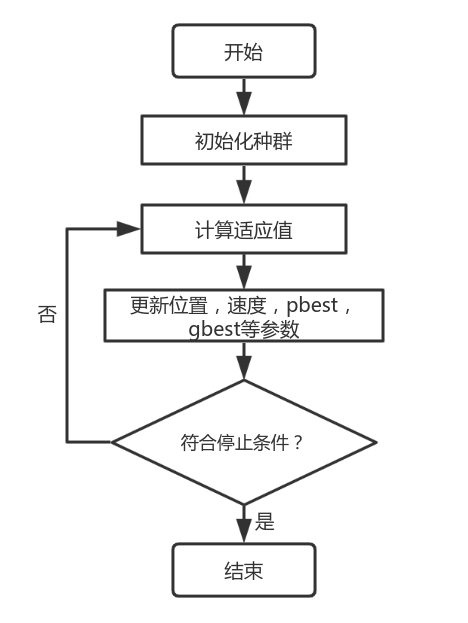
\includegraphics[width = 0.5\textwidth]{pso}
    \caption{粒子群算法流程图}
    \label{fig:pso}
  \end{figure}

  \subsection{布谷鸟搜索算法}
    布谷鸟搜索算法(Cuckoo Search, CS)是Yang和Deb于2009年提出的新兴启发算法,其流程图如图\ref{fig:cs}所示。该算法通过模拟布谷鸟寄生育雏行为,在可行域中通过Levy飞行寻找合适的鸟巢,来找到较优解。该算法有三条理想化的规则:
    \begin{enumerate}
      \item {每只布谷鸟每次下一个蛋,并将其放入随机选择的巢中。}
      \item {具有优质蛋的最佳巢会被带到下一代。}
      \item {可用的寄主巢数量是固定的,且寄主以概率$P_a\in(0,1)$发现布谷鸟放的蛋。在这种情况下,寄主可以消灭该蛋或放弃旧巢另建新巢。}
    \end{enumerate}

    CS中有两种更新方式,一种是布谷鸟寻找宿主鸟巢的Levy飞行:
    \begin{align}
      x_{i+1}=x_i+\alpha\otimes Levy(\beta)
    \end{align}
    其中,$\alpha$是步长缩放因子, $Levy(\beta)$是Levy飞行路径。

    另一种是寄主以概率$P_a$发现外来鸟蛋后,采用随机方式重新建巢:
    \begin{equation}
      x_{i+1}=x_i+r\otimes Heaviside(P_a-\varepsilon)\otimes(x_t-x_k)
    \end{equation}
    其中,$r,\varepsilon$是服从均匀分布的随机数,$Heaviside()$是跳跃函数,$x_t,x_k$是其他任意的两个鸟巢。
    \begin{figure}[htbp]
      \centering
      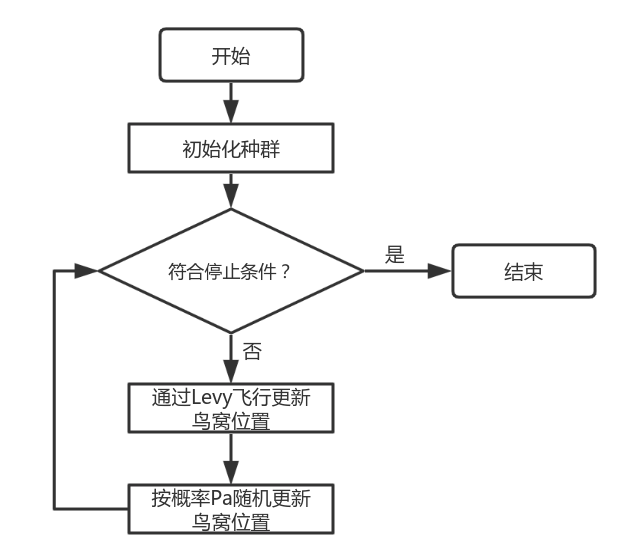
\includegraphics[width = 0.7\textwidth]{cs}
      \caption{布谷鸟算法流程图}
      \label{fig:cs}
    \end{figure}

  \subsection{萤火虫算法}
  萤火虫算法(Firefly Algorithm,FA)是Yang于2008年提出的一种启发算法,其流程图如图\ref{fig:fa}所示。把空间各点看成萤火虫,利用发光强的萤火虫会吸引发光弱的萤火虫的特点,在发光弱的萤火虫向发光强的萤火虫移动的过程中,完成位置的迭代,从而找出最优位置。算法有以下三条假设:
  \begin{enumerate}
    \item {萤火虫不分性别,这样一个萤火虫将会吸引到所有其他的萤火虫。}
    \item {吸引力与它们的亮度成正比,对于任何两个萤火虫,不那么明亮的萤火虫被吸引,因此移动到更亮的一个,然而,亮度又随着其距离的增加而减少。}
    \item {如果没有比一个给定的萤火虫更亮的萤火虫,它会随机移动。}
  \end{enumerate}
  萤火虫的相对荧光亮度计算方式:
  \begin{align}
    I=I_0e^{-\gamma r_{ij}}
  \end{align}
  其中, $I_0$表示最亮萤火虫的亮度,即自身($r=0$处)荧光亮度,与目标函数值相关,目标函数值越优,自身亮度越高;$\gamma$表示光吸收系数,因为荧光会随着距离的增加和传播媒介的吸收逐渐减弱,所以设置光强吸收系数以体现此特性,可设置为常数;$r_{ij}$表示萤火虫$i$与$j$之间的距离。 

  当萤火虫$i$的相对亮度小于萤火虫$j$时,向萤火虫$j$靠拢。位置的更新方式为:
  \begin{align}
    \beta(r)&=\beta_0e^{-\gamma r_{ij}^2} \\
    x_i&=x_i+\beta(x_j-x_i)+\alpha(rand-1/2)
  \end{align}
  其中, $\beta_0$表示最大吸引度,即光源处($r=0$处)的吸引度。$\alpha$为步长因子,$rand$为[0,1]上服从均匀分布的随机因子。

  \begin{figure}[htbp]
    \centering
    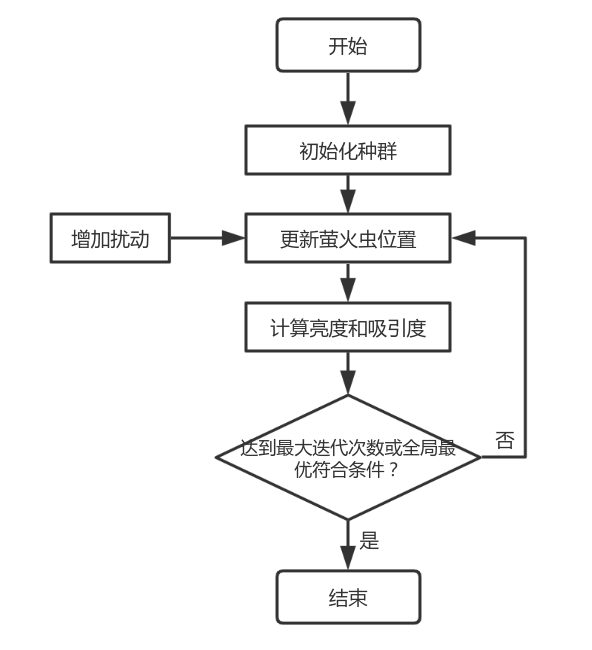
\includegraphics[width = 0.6\textwidth]{fa}
    \caption{萤火虫算法流程图}
    \label{fig:fa}
  \end{figure}

  \subsection{细菌觅食算法}
  细菌觅食算法(Bacterial Foraging Optimization,BFO)由Passino于2002年提出,其流程图如图\ref{fig:bfo-2}所示。通过模拟大肠杆菌菌落的觅食行为,不断地使用鞭毛游动和翻转,最终躲开有毒的地方并找到营养度高的位置,如图\ref{fig:bfo}所示。算法分为趋向性操作(趋化操作)、复制操作和迁徙操作。
  \begin{figure}[htbp]
    \centering
    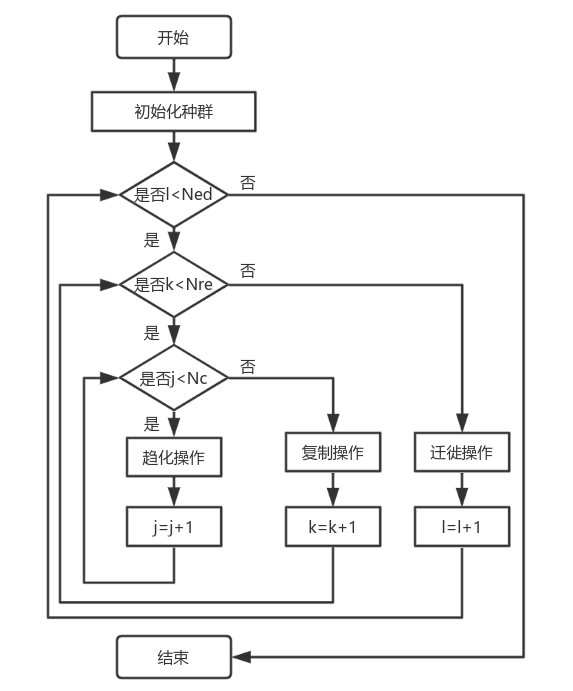
\includegraphics[width = 0.5\textwidth]{bfo-2}
    \caption{细菌觅食算法流程图}
    \label{fig:bfo-2}
  \end{figure}
  
  \begin{figure}[htbp]
    \centering
    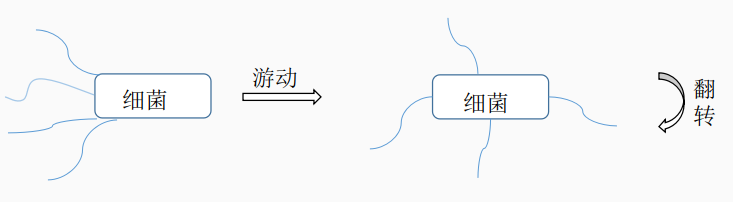
\includegraphics[width = 0.7\textwidth]{bfo.png}
    \caption{细菌的游动和翻转}
    \label{fig:bfo}
  \end{figure}

  \begin{enumerate}
    \item[1.] 趋向性操作。 
    这一操作模拟得是大肠杆菌的游动和翻转。在营养度高的地区,细菌会更多地游动,在营养度低的地区,细菌会更多地翻转,以逃出该地区。设细菌的种群规模为$S$,维度为$n$。细菌的觅食行为可以用以下公式表示:
    \begin{align}
      \theta(i,j+1,k,l) &= \theta(i,j,k,l) + C(i) \times \phi(i,j) \\
      \phi(i,j) &= \frac{\Delta(i)}{\sqrt{\Delta^T(i)\Delta(i)}}
    \end{align}
    其中,$\theta(i,j,k,l)$表示细菌在第$j$次趋向性操作,第$k$次复制操作和第$l$次迁徙操作时的位置。$C(i)$是细菌$i$的趋向性步长。$\phi(i,j)$表示细菌在第$j$次趋向性操作时的随机方向的单位向量。$\Delta(i)$为随机向量。

    \item[2.] 复制操作。
    复制操作的目的是将表现不好的细菌淘汰掉。首先,对种群按适应度排序,然后,前一半的细菌会复制一份覆盖后一半的细菌。保持种群数量不变的同时,实现优胜劣汰的机制。

    \item[3.] 迁徙操作。
    在生物观察中发现,随着某些条件的改变,可能会使该地区的细菌突然死亡或迁移。算法通过迁徙操作模拟这一现象,提高种群的多样性。细菌会以一定的概率被清除,并随机生成一个新的细菌。
    
  \end{enumerate}

\section{本章小结}
生物信息学中,通过双聚类分析对基因表达数据进行挖掘,希望找到在对应条件下紧密相关的基因集合。本章主要对基因表达数据上的双聚类的相关知识进行了阐述,先是介绍了基因表达数据的重要性以及特点;然后对双聚类的定义、类型和结构进行了描述;接下来对常用的质量评价指标以及生物评价指标进行了简要介绍,以及把双聚类算法分为了基于质量评价指标的和基于模型的两种;最后简要说明了本文用到的几种群智能算法。

% !Mode:: "TeX:UTF-8"
\chapter{基于CS和FA的混合双聚类算法}
元启发式算法在双聚类领域的应用取得了很不错的效果,但元启发式算法本身的缺陷也会影响着双聚类的质量。一般来说,不同的算法有不同的使用范围,一个算法很难做到兼顾全局寻优与快速收敛。比如,布谷鸟算法具有较强的全局搜索能力,而在局部搜索却表现欠佳;萤火虫算法跟布谷鸟算法却刚好相反。全局寻优能力使得算法在寻在双聚类中能够找到更多样的结果,提高了覆盖率;局部寻优能力能够指导算法找到生物意义更加明确的双聚类结果。本文结合布谷鸟算法和萤火虫算法,提出一种混合的元启发式双聚类算法(CS-FA Biclustring,CSFAB),并将CSFAB算法在四个基因表达数据与其他常用的双聚类算法进行了质量验证指标和生物验证指标的比较。

\section{混合双聚类算法分析}
    \subsection{编码设计}
    给定基因表达矩阵$E(X,Y)$,比特串$x_p = (g_1,\dots,g_i,\dots,g_m,s_1,\dots,s_j,\dots,s_n)$,$ p=1,\dots,N, $ 被用来表示一个双聚类或子矩阵$E(I,J)$。其中, $N,m,n$分别是种群数量,$E$的基因数目和样本数目。当$E$中第$i$个基因或第$j$个样本被选为$E(I,J)$时,$g_i=1$或$s_j=1$,否则,$g_i=0$或$s_j=0$,$1\le i \le m$ 且$1\le j \le n$。

    原始的群智能算法的解(粒子,鸟巢,萤火虫)都是多维的连续值,需要映射成对应的比特串后才能用来表示双聚类。通常的做法就是设置上限为1,下限为0,然后判断是否大于0.5,将实数值映射成比特值。如下图所示:
    \begin{figure}[htbp]
        \centering
        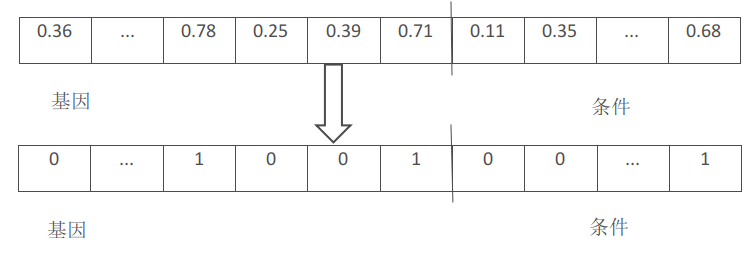
\includegraphics[width = 0.7\textwidth]{coding.png}
        \caption{将连续的解映射为双聚类}
        \label{fig:encoding}
    \end{figure}

    \subsection{适应值函数设计}\label{sec:fitness}
    优化算法需要知道优劣的评价标准,在群智能算法中一般称之为适应值。我们需要设计一个适应值函数,用来得到一个解的质量,从而在解与解之间以及算法之间进行比较。正如\ref{section:qualityEval}小节提到的,MSR是最主要也是最直观的质量评价指标,同时双聚类的体积也是衡量好坏的标准之一。一般来说,体积越大的双聚类MSR会相应的变大,而我们希望找到体积大但是MSR较小的双聚类。所以,需要在保持两者之间平衡的同时,能够引导双聚类算法找到更优的解。对于双聚类$B(I,J)$,其适应值为:
    \begin{align}
      f(B) &= MSR(B) + \frac{\lambda}{GV(B)} +\frac{\mu}{CV(B)} \\
      GV(B) & = |I| \\
      CV(B) & = |J|
    \end{align}
    其中,$GV(B)$,$CV(B)$分别是$B(I,J)$中基因和实验条件的容量。$\lambda,\mu$是针对量纲不同问题,$\lambda,\mu$越大则GV和CV对适应值的影响越大,其值视数据集的情况而定。
    
    \subsection{混合方案设计}\label{sec:three}
    大致有两种策略将两个算法混合,顺序执行策略和嵌套策略。第一种策略是将一个算法的结果作为另一个算法的输入,特点是两个算法前后互不影响。Nepomuceno 等将SEBI的结果输入到SSB算法中,进一步提高双聚类的质量。第二种策略是将两个算法的揉合到一起,将某一个算法作为局部功能嵌入到另一个算法中,这时两种算法前后不是独立的。例如,Bryan 等将CC算法的局部搜索功能作为SAB算法的一步,以提高双聚类的容量。基于上述二种策略,可有如下三种方案:
    \begin{enumerate}
       \item[(1)] 顺序执行CS-FA:这种方案可以看作将FAB算法的随机初始化替换成CSB算法,先使用CSB算法生成双聚类,然后使用FAB算法进一步提高双聚类的质量,如算法\ref{alg:cs-fa}所示。
        \begin{algorithm}[htbp]
        \caption{CS-FA混合方案} \label{alg:cs-fa}
        % \AlgoBiCaption{这是一个简短的算法中文图题}{This is the English caption of the algorithm}
        \KwIn{$n \times m$的基因表达矩阵E,弃巢比例p,种群大小N,光吸收系数$\gamma$,最大吸引度$\beta_0$,步长因子$\alpha$,最大迭代次数Iter}
        \KwOut{一个满足条件的双聚类B}%
        P = Initialization(E, N) //初始化种群 \\
        $P_{CS}$ = CSB(P,E,p,Iter) \\
        $P_{CS-FA}$ = FAB(P,E,$\gamma$,$\beta_0$,$\alpha$,Iter) \\
        B = Best($P_{CS-FA}$) \\
        return B
        \end{algorithm}

       \item[(2)] 顺序执行FA-CS:与第一种方案刚好相反,将CSB算法的随机初始化改为FAB算法,如算法\ref{alg:fa-cs}所示。
        \begin{algorithm}[htbp]
        \caption{FA-CS混合方案}\label{alg:fa-cs}
        \KwIn{$n \times m$的基因表达矩阵E,弃巢比例p,种群大小N,光吸收系数$\gamma$,最大吸引度$\beta_0$,步长因子$\alpha$,最大迭代次数Iter}
        \KwOut{一个满足条件的双聚类B}%

        P = Initialization(E, N) //初始化种群 \\
        $P_{FA}$ = FAB(P,E,$\gamma$,$\beta_0$,$\alpha$,Iter) \\
        $P_{FA-CS}$ = CSB(P,E,p,Iter) \\
        B = Best($P_{FA-CS}$) \\
        return B \\
        \end{algorithm}
       \item[(3)] 嵌套执行CS-FA:该方案在每一次迭代都会执行CS操作和FA操作,并且采用竞标策略保留两次操作中最优的个体。
        \begin{algorithm}[htbp]
        \caption{CSFA混合方案}\label{alg:csfa}
        \KwIn{$n \times m$的基因表达矩阵E,弃巢比例p,种群大小N,光吸收系数$\gamma$,最大吸引度$\beta_0$,步长因子$\alpha$,最大迭代次数Iter,最大早熟次数maxEarlyStopCnt}
        \KwOut{一个满足条件的双聚类B}%
        i = 1 \\
        earlyStopCnt = 0 \\
        $B_{old}$ = INF \\
        $P_{fa}$ = Initialization(E, N) //初始化种群 \\
        \Do{(i<=Iter AND earlyStopCnt< maxEarlyStopCnt)}
        {
            $P_{cs}$, $best_{cs}$ = csIter($P_{fa}$, E, p) \\
            $P_{fa}$, $best_{fa}$ = faIter($P_{cs}$, E, $\gamma$,$\beta_0$,$\alpha$) \\
            B = Best( $best_{cs}$, $best_{fa}$) \\
            earlyStopCnt = EarlyStop(earlyStopCnt, B, $B_{old}$)
            $B_{old}$ = B \\
            i++
        }
        return B
        \end{algorithm}
    \end{enumerate}
    \subsection{停止条件}
    算法的停止条件是达到最大的迭代次数或者种群中最优双聚类的质量已经有一定的时间不再提升,后一种情况称为early stopping。通过EarlyStop函数来实现,当新的最优适应值相比较上一代的最优适应值几乎没有变化时,将earlyStopCnt加一,否则置零。
    \begin{algorithm}[htbp]
    \caption{EarlyStop函数}
    \SetAlgoLined
    \KwIn{earlyStopCnt, 新的最优适应值$f_{new}$,旧的最优适应值$f_{old}$}
    \KwOut{新的earlyStopCnt}%
        \uIf{ |$f_{new}$ - $f_{old}$| < $f_{new}/1000$}{earlyStopCnt++\;}
        \Else{earlyStopCnt = 0}
        return earlyStopCnt 
    \end{algorithm}

\section{实验环境及基因表达数据}
本节主要介绍实验所用到的软硬件环境和数据,后面章节的实验所用的环境和数据与本节相同,将不再赘述。
    \subsection{实验环境}
    本文提出的CSFAB双聚类算法与其他用来比较的算法均是用Matlab语言实现,并运行在Matlab R2018b环境中。对于双聚类结果的生物验证,是用R语言的clusterProfiler包得到的。所有代码都运行在64位的Ubuntu 18.04操作系统上,CPU是intel i7-9700K,内存大小为16G。

    \subsection{基因表达数据}
    不同的双聚类算法采取不同的搜索策略,有不同的侧重。为了全面的评估本文所提出的算法,本文选择了四个数据量各不同的数据集,如表\ref{tab:data}所示。
    \begin{table}[htbp]
    \caption{本文所用的基因表达数据集的相关信息}\label{tab:data}
    % \bicaption[table1]{}{符合研究生院绘图规范的表格}{Table$\!$}{Table in agreement of the standard from graduate school}
    \vspace{0.5em}\centering\wuhao
    \begin{tabular}{cccccc}
    \toprule[1.5pt]
    数据名缩写 & 数据全名 & 基因数量 & 条件数量 & $\lambda$& $\mu$ \\
    \midrule[1pt]
    Yeast Cell & Yeast cell cycle & 5847& 50 & 2.0E05 &  2.0E03\\
    BCLL & B-cell chronic lymphocytic leukemia& 12815& 21 & 1.0E04 & 1.0E03\\
    RatStrain & Rat multiple tissue in strain& 7751& 122 & 6.0E05 & 1.0E04\\
    PBC & Primary breast cancer& 21225& 286 & 3.0E06 & 4.0E04\\
    \bottomrule[1.5pt]
    \end{tabular}
    \end{table}
    这些基因表达数据集都是来自GEO数据库,编号分别为GDS2350,GSE2403,GSE952,GSE2034。$\lambda$和$\mu$均为经验值。本文使用Python的GEOParse包和Pandas包在基因维度上对数据进行了Min-max Normalization,缩放到[0,1]区间并乘以100。计算公式如下。
    \begin{equation}
        x^{\prime} = \frac{x - min(x)}{max(x) - min(x)} \times 100
    \end{equation}
    其中,$x$为基因表达数据的某一行,也就是该基因在所有条件下的表达水平。

\section{实验结果及分析}
本节主要内容为三种混合方案的性能分析比较,然后在四个基因表达数据上对各双聚类算法进行测试,最后在质量验证指标和生物验证指标对各算法进行讨论分析。
    \subsection{混合方案比较}
    为了确定\ref{sec:three}节中提到的三种方案中,哪种更适合双聚类分析,本文在BCLL数据集上,使用\ref{sec:fitness}节中定义的适应值函数,分别对三种方案进行了100次实验,得到相应的双聚类。因为在算法中使用到了三个指标,为了减少偏向性,同时对相关指数RI和HV-Score共五个指标计算其平均值和标准差,如表\ref{tab:three}所示。由表\ref{tab:three}可知,前两种混合方案能够使双聚类的体积增加一些,在HV-Score 和样本个数指标上,三种策略的差别并不大,但是嵌套执行方案在MSR和RI上均有明显的优势。所以,本文抛弃了顺序执行方案,并将嵌套执行方案命名为CSFAB。

    \begin{table}[htbp]
        \caption{三种混合方案在BCLL数据集上的质量评价指标}\label{tab:three}
        \vspace{0.5em}\centering\wuhao
        \begin{tabular}{cccccc}
        \toprule[1.5pt]
         & 基因个数 & 样本个数 & MSR & RI& HV-Score \\
        \midrule[1pt]
        CS-FA  &$\bm{6093.88\pm 39.12}$& $\bm{8.03\pm 0.99$}&$296.212\pm 7.26$ & $0.019\pm 0.003$&  $0.994\pm 0.001$ \\
        FA-CS  &$6044.54\pm 51.53$& $7.54\pm 0.65$&$307.616\pm 14.17$ & $0.006\pm 0.005$&  $0.995\pm 0.001$ \\
        CSFA   &$5992.93\pm 61.52$& $8.0\pm 0.0$&\bm{$277.049\pm 2.97$} & $\bm{0.031\pm 0.003$}& \bm{$0.994\pm 0.0007$} \\
        \bottomrule[1.5pt]
        \end{tabular}
    \end{table}

    \subsection{CSFAB的质量验证指标比较分析}
    为了较公平和全面地衡量本文提出的CSFAB算法的有效性,本文选择了采用相同的编码方案和适应值函数的萤火虫算法,布谷鸟搜索算法和粒子群算法作为对比算法,并分别命名为FAB,CSB,PSOB。表\ref{tab:gv}和表\ref{tab:cv}分别为各算法在各数据集上的基因容量和样本容量的平均值和标准差。同时,为了评价算法的多样性,图\ref{fig:coverRate}展示了各算法在不同基因表达数据集上的覆盖率。图\ref{fig:msr}和图\ref{fig:ri}给出了各算法在在四个数据集上MSR以及RI的箱线图。
    
    从表\ref{tab:gv}可以看出,PSOB在BCLL数据集上表现最优,而CSFAB在其他三个数据集上均取得了最大的基因容量。而表\ref{tab:cv}表明,在样本容量方面,CSFAB表现平平,仅在量级最大的PBC中比另外三个算法更优,其他三个数据集均为FAB算法最优。但在BCLL中,各算法的表现相差不大。实验数据说明,在数量级比较大时,CSFAB算法更占优势。图\ref{fig:coverRate}可知,无论是在什么量级的数据中,相比其他算法,CSFAB算法总能找到更多样化的双聚类。

    \begin{table}[htbp]
        \caption{CSFAB等四个算法的基因容量平均值与标准差}\label{tab:gv}
        \vspace{0.5em}\centering\wuhao
        \begin{tabular}{ccccc}
        \toprule[1.5pt]
         & Yeast Cell & BCLL & RatStrain & PBC \\
        \midrule[1pt]
        CSB & $2974.42\pm 41.57$& $6075.06\pm 50.18$& $3929.93\pm 47.22$& $10781.59\pm 80.67$\\
        FAB & $3034.14\pm 40.78$& $6053.57\pm 58.17$& $4126.25\pm 39.74$& $11268.66\pm 61.56$\\
        CSFAB & \bm{$3093.02\pm 37.56$}& $5992.93\pm 61.52$&\bm{$4193.04\pm 48.38$}& $\bm{11539.04\pm 82.86$}\\
        PSOB & $3030.74\pm 41.14$ & $\bm{6093.41\pm 49.89$}& $4094.83\pm 43.77$& $11052.69\pm 78.39$\\
        \bottomrule[1.5pt]
        \end{tabular}
    \end{table}

    \begin{table}[htbp]
        \caption{CSFAB等四个算法的样本容量平均值与标准差}\label{tab:cv}
        \vspace{0.5em}\centering\wuhao
        \begin{tabular}{ccccc}
        \toprule[1.5pt]
         & Yeast Cell & BCLL & RatStrain & PBC \\
        \midrule[1pt]
        CSB & $18.82\pm 0.71$& $7.86\pm 0.40$& $71.96\pm 3.96$& $202.79\pm 5.31$\\
        FAB &\bm{$23.01\pm 2.67$}&\bm{$8.03\pm 0.30$}& \bm{$80.59\pm 2.82$}& $259.41\pm 5.09$\\
        CSFAB &$18.35\pm 0.47$ & $8.0\pm 0.0$& $76.01\pm 1.79$& $\bm{267.79\pm 2.65$}\\
        PSOB &$22.66\pm 3.23$ &$7.98\pm 0.58$ & $77.08\pm 3.44$& $220.94\pm 6.76$\\
        \bottomrule[1.5pt]
        \end{tabular}
    \end{table}

    \begin{figure}[htbp]
        \centering
        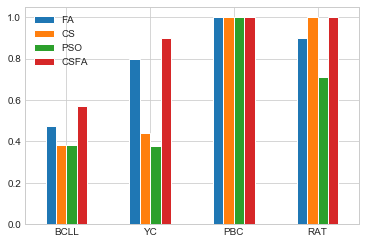
\includegraphics[width = 0.6\textwidth]{coverRate}
        \caption{CSFAB等四个算法的覆盖率}
        \label{fig:coverRate}
    \end{figure}
    从图\ref{fig:msr}可以看出,CSFAB在全部的数据集上都找得了MSR最小的双聚类,并且优势明显。一方面,这是由于适应值函数中MSR所占的比重是相对较大的,这也解释了在样本容量上,CSFAB表现并不突出;另一方面,结合Lavy飞行和萤火虫,使得算法有了更强的寻优能力。值得一提的是,CSFAB算法的四分位间距是最小的,这一现象说明了CSFAB算法的稳定性。为了减少对MSR的倾向性,图\ref{fig:ri}展示了没有参与适应值函数的评价指标相关系数RI,值得注意的是,该指标越大则质量越好。从图中可以看出,CSFAB仅在Yeast Cell数据集紧跟在PSOB,FAB之后,另外三个数据集都取得了最优的结果。
    \begin{figure}[htbp]
    \setlength{\subfigcapskip}{-1bp}
    \centering
    \begin{minipage}{.8\textwidth}
    \centering
    \subfigure{\label{fig:msr_bcll}}\addtocounter{subfigure}{-2}
    \subfigure{\subfigure[BCLL]{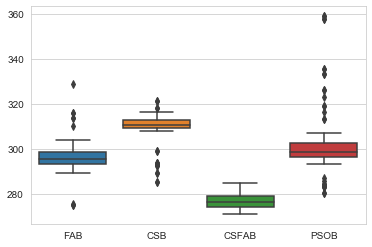
\includegraphics[width=0.4\textwidth]{msr_bcll}}}
    \hspace{.2em}
    \subfigure{\label{fig:msr_yc}}\addtocounter{subfigure}{-2}
    \subfigure{\subfigure[Yeast Cell]{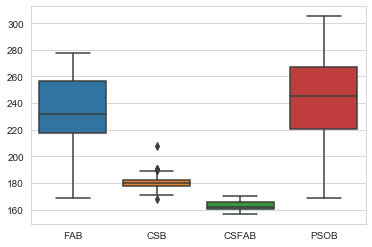
\includegraphics[width=0.4\textwidth]{msr_yc}}}
    \end{minipage}
    \centering
    \begin{minipage}{.8\textwidth}
    \centering
    \hspace{.2em}
    \subfigure{\label{fig:msr_pbc}}\addtocounter{subfigure}{-2}
    \subfigure{\subfigure[PBC]{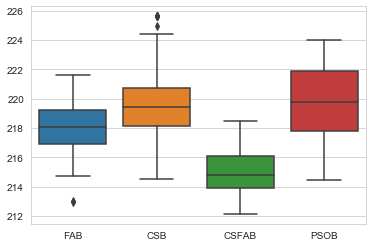
\includegraphics[width=0.4\textwidth]{msr_pbc}}}
    \hspace{.2em}
    \subfigure{\label{fig:msr_rat}}\addtocounter{subfigure}{-2}
    \subfigure{\subfigure[RatStrain]{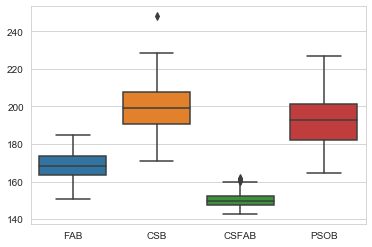
\includegraphics[width=0.4\textwidth]{msr_rat}}}
    \end{minipage}
    \vspace{0.2em}
    \caption{CSFAB等四个算法的MSR}
    \label{fig:msr}
    \end{figure}

    \begin{figure}[htbp]
    \setlength{\subfigcapskip}{-1bp}
    \centering
    \begin{minipage}{.8\textwidth}
    \centering
    \subfigure{\label{fig:ri_bcll}}\addtocounter{subfigure}{-2}
    \subfigure{\subfigure[BCLL]{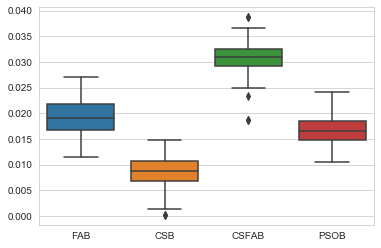
\includegraphics[width=0.4\textwidth]{ri_bcll}}}
    \hspace{.2em}
    \subfigure{\label{fig:ri_yc}}\addtocounter{subfigure}{-2}
    \subfigure{\subfigure[Yeast Cell]{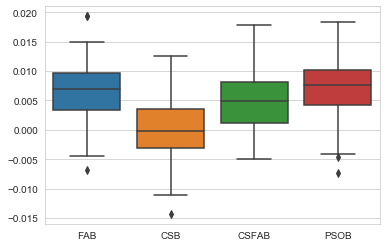
\includegraphics[width=0.4\textwidth]{ri_yc}}}
    \end{minipage}
    \centering
    \begin{minipage}{.8\textwidth}
    \centering
    \hspace{.2em}
    \subfigure{\label{fig:ri_pbc}}\addtocounter{subfigure}{-2}
    \subfigure{\subfigure[PBC]{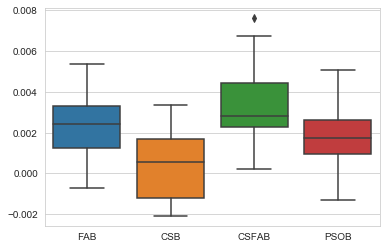
\includegraphics[width=0.4\textwidth]{ri_pbc}}}
    \hspace{.2em}
    \subfigure{\label{fig:ri_rat}}\addtocounter{subfigure}{-2}
    \subfigure{\subfigure[RatStrain]{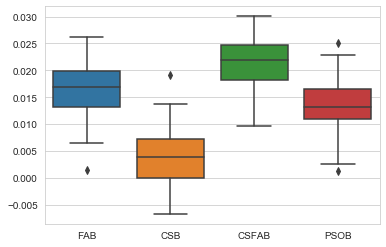
\includegraphics[width=0.4\textwidth]{ri_rat}}}
    \end{minipage}
    \vspace{0.2em}
    \caption{CSFAB等四个算法的RI}
    \label{fig:ri}
    \end{figure}

    以上分析表明,尽管CSFAB在样本容量方面没有取得足够的优势,但是在基因容量和MSR以及RI上都取得了显著的成绩。不过,对于基因表达数据的一个双聚类,还需要以生物质量指标来判断优劣。

    \subsection{CSFAB的生物验证指标比较分析}
    虽然CSFAB在质量评价指标上表现不俗,但是对于双聚类来说,还是要找到具有生物意义的双聚类才行。因此,我们对实验中得到的双聚类进行了GO富集分析,并通过图表的方式展示。表\ref{tab:we}给出了CSFAB等四个算法的WEScore平均值与标准差。

    由表\ref{tab:we}可知,在RatStrain和PBC这两个大数据集上,CSFAB算法是最优的,而且在Yeast Cell数据集上是次优的,仅比最优的FAB低了2.5个百分点。这充分说明CSFAB算法更适合在大规模的数据上搜索相对其它算法难以搜索到的双聚类。

    \begin{table}[htbp]
        \caption{CSFAB等四个算法的WEScore平均值与标准差}\label{tab:we}
        \vspace{0.5em}\centering\wuhao
        \begin{tabular}{ccccc}
        \toprule[1.5pt]
         & Yeast Cell & BCLL & RatStrain & PBC \\
        \midrule[1pt]
        CSB & $43.59\pm 7.45$& \bm{$231.93\pm 14.10$}& $124.20\pm 44.52$& $137.90\pm 10.54$\\
        FAB &\bm{$45.76\pm 8.34$}&$230.55\pm 14.91$& $119.85\pm 41.61$& $149.24\pm 9.22$\\
        CSFAB &$44.59\pm 7.17$ & $228.71\pm 14.55$& \bm{$124.91\pm 42.06$}& $\bm{153.49\pm 12.73$}\\
        PSOB &$43.27\pm 8.03$ &$230.89\pm 14.92$ & $115.30\pm 38.60$& $143.24\pm 8.30$\\
        \bottomrule[1.5pt]
        \end{tabular}
    \end{table}
    图\ref{fig:meanP}为CSFAB等四个算法的meanPValue。与WEScore吻合的是,数据集越大,则CSFAB算法的表现越好。在规模最大的PBC数据集上,CSFAB的优势最为明显。同样在Yeast Cell数据集上是次优的,仅比最优的FAB低了0.7个百分点。

    \begin{figure}[htbp]
    \setlength{\subfigcapskip}{-1bp}
    \centering
    \begin{minipage}{.8\textwidth}
    \centering
    \subfigure{\label{fig:meanP_bcll}}\addtocounter{subfigure}{-2}
    \subfigure{\subfigure[BCLL]{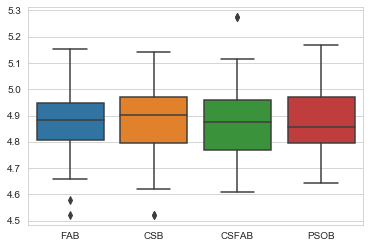
\includegraphics[width=0.4\textwidth]{meanP_bcll}}}
    \hspace{.2em}
    \subfigure{\label{fig:meanP_yc}}\addtocounter{subfigure}{-2}
    \subfigure{\subfigure[Yeast Cell]{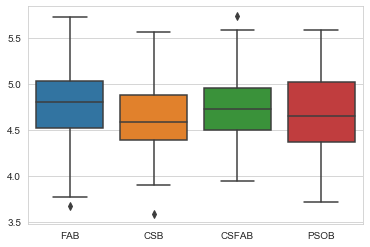
\includegraphics[width=0.4\textwidth]{meanP_yc}}}
    \end{minipage}
    \centering
    \begin{minipage}{.8\textwidth}
    \centering
    \hspace{.2em}
    \subfigure{\label{fig:meanP_pbc}}\addtocounter{subfigure}{-2}
    \subfigure{\subfigure[PBC]{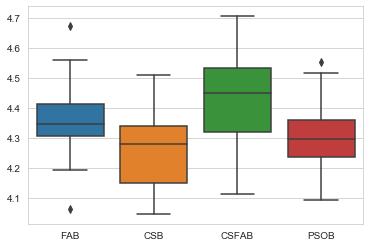
\includegraphics[width=0.4\textwidth]{meanP_pbc}}}
    \hspace{.2em}
    \subfigure{\label{fig:meanP_rat}}\addtocounter{subfigure}{-2}
    \subfigure{\subfigure[RatStrain]{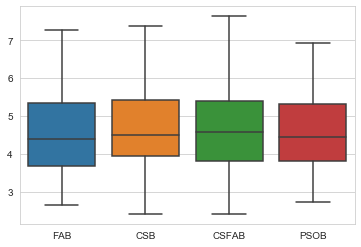
\includegraphics[width=0.4\textwidth]{meanP_rat}}}
    \end{minipage}
    \vspace{0.2em}
    \caption{CSFAB等四个算法的meanPValue}
    \label{fig:meanP}
    \end{figure}

\section{本章小结}
本文为了解决元启发式算法在双聚类时覆盖率不高和生物意义不明显的问题,提出了将CS算法和FA算法结合的CSFAB算法。首先提出了三种混合的方案,经实验比较后选择了嵌套执行的方案。然后,在四个数据集上对CSB,FAB和PSOB等四个算法进行了讨论分析。最后,实验证明,CSFAB不仅提高了双聚类的多样性,而且保证了其生物意义,在规模大的数据集上更加明显。


% !Mode:: "TeX:UTF-8"
\chapter{基于BFO的多目标优化双聚类算法}

\section{算法描述}

\section{实验结果及分析}

\section{本章小结}

\chapter{总结与展望}
\section{论文的工作总结}
科学技术的进步使得人类有了更多的途径来认知事物,而数据则是人类认知事物的特殊媒介。随着高新科技的迅猛发展,越来越多的数据被产生出来,挖掘出蕴藏在数据中的价值,将带来巨大的经济和社会价值。而基因表达数据作为一种特殊的数据,保存着生命密码,能够帮助人们更加了解自身和自然,对医疗以及生态保护都有长远的意义。因为生物体中的细胞种类繁多和基因之间互相调控等方面的原因,基因表达数据有着较为复杂,体量大和增长速度快的特点。因此对于基因表达数据的研究一直是生物信息学领域的难点和重点。

聚类一直是人们分析数据时常用的手段之一。而传统的聚类方法无法找到基因表达数据中的局部模式,所以双聚类分析成为了最主要的挖掘工具。在有的双聚类分析算法中,基于元启发式的优化算法和多目标优化被应用到寻找双聚类。因此,本文以解决双聚类算法中常见的问题,如质量评价不高和生物意义不明显,为出发点,运用算法融合和多目标优化的手段,做了一些总结和探索性的工作,主要包括:
\begin{itemize}
    \item[1.]{介绍了基因表达数据双聚类分析的研究背景和意义。然后,对基因表达数据双聚类分析的基础概念和和数学定义进行了阐述,如基因表达数据的数学模型,双聚类的相关概念,常见的双聚类分析方法的分类以及常用的双聚类验证指标。最后,对于本文所涉及的群智能算法也进行了说明}  

    \item[2.]{本文基于布谷鸟算法中的levy飞行和萤火虫算法中的亮度吸引作用,将两个算法嵌套融合,提出了CSFAB双聚类算法。然后讨论了适应值函数,混合方案和停止条件,并通过实验证明了所提出算法具有更高的全局搜索能力和收敛能力,达到预期目标。}

    \item[3.]{本文从多目标优化的角度,对细菌觅食算法进行了相应的设计,如种群的趋化操作和迁徙操作。基于多目标细菌觅食算法,提出MOBFOB双聚类算法。算法对双聚类的均方残差和容量同时优化,使得成对立关系的指标都能得到优化,最终得到占优的双聚类。实验证明,MOBFOB算法能都有效地找到高质量的双聚类。}
    
\end{itemize}
\section{后续工作展望}
基因表达数据的双聚类分析是一个很大且复杂的研究方向。由于时间和条件有限,本文仅仅是对群智能算法做了一些工作。本工作仍有不少问题需要进一步的研究,包括:
\begin{itemize}
    \item [1.]{由于性能的关系,质量评价指标和生物意义被分别考虑。优化算法也只是根据质量评价指标来寻优,这与基因表达数据双聚类分析的目的是存在一定的偏差的。最近,Nepomuceno 等使用SSB双聚类算法直接以GO注释信息来指导搜索,取得了一定的效果,但仍有很多不足。如何更好地直接利用GO信息来需找双聚类,还需要进一步的研究。}

    \item [2.]{二维基因表达数据无法全面的记录所需要的信息。目前所用的基因表达数据都是二维矩阵形式的,而现实中,基因的表达是有时序关系的。只有将时间序列这一维度引入进来,才能够更完全更科学地找到双聚类。}

    \item [3.]{将算法优势互补的方法不止融合一种,还可以通过集成的方法来提高双聚类结果的质量。在机器学习领域,集成能够将多个相对较弱的模型组合成一个效果更好的模型,如随机森林算法,XGBoost算法等。如何将不同的双聚类算法集成为一个效果更好的算法,仍处于研究初始阶段,这指明了下一步的研究方向。}
    
\end{itemize}


\backmatter
%硕博书序
% % !Mode:: "TeX:UTF-8" 
\begin{conclusions}
\section*{一、本文工作总结}
信息科学技术的持续创新与发展使得互联网音乐盛行。各个音乐平台的不断更新和优化,纷纷竞争着迎合市场需求,争取留住老用户,赢得新用户。音乐流行趋势直接决定了音乐未来走势,这都需要音乐平台的开发者发掘新的算法和技术,让用户体验更好,从而增加平台收益。本文切实从互联网企业的实际问题出发,针对互联网音乐平台竞争力的不断增加的问题,综合分析用户的行为记录和歌手歌曲数据,预测歌手们的播放量即进行预测音乐流行趋势,以把握未来一段时间内的流行歌曲、流行歌手,这对于音乐平台来说,预先把握了流行歌曲,那么就会获得用户,增长收益;对于歌手而言,可以被提前挖掘出来,为自己美好的发展作准备;对于用户来说,能听到精准预测得到的流行歌手的流行歌曲,会有很满意的体验。

目前,对于互联网音乐流行趋势预测的研究主要存在以下几种模型和算法:
\begin{itemize}
    \item[(1)] {利用神经网络模型进行音乐流行趋势预测。这种模型的构建速度有待提高,对实验环境要求高,使得耗费时间多,预测效果也一般。而且人工神经网络需要大量的参数,那么参数的设定对于实验的结果影响较大,且工作量繁杂。}
    \item[(2)] {利用支持向量机模型的音乐流行趋势预测。这个模型对于大规模的数据训练比较困难,无法直接支持多分类。模型的学习能力有限,对于核函数的高维映射解释力不强,尤其是径向基函数。对缺失数据敏感。对于处理大量的互联网音乐数据来说,不是一个好的选择。}
    \item[(3)] {利用ANN+SVM组合模型进行预测音乐流行趋势。这种模型比的单一的模型效果要好,但仍然不能很好的学习多维特征,处理大量数据训练能力不佳,因此对音乐流行趋势预测的效果提升不高。}
    \item[(4)] {通过GBDT模型进行音乐流行趋势预测。模型对更换数据集较为敏感,对于任意足够大,且总体参数不稳定的数据集,预测效果就差很多。模型对自身参数也敏感,不能保证参数在一定范围内的变化不敏感,预测效果一般。}
\end{itemize}

本文针对音乐流行趋势预测模型目前的研究成果所面临的挑战,研究了基于随机森林算法预测音乐流行趋势模型和爆增型歌曲衰减模型,基于LSTM时间序列预测音乐流行趋势模型以及基于ARIMA时间序列预测音乐流行趋势模型。本文主要贡献有以下几点:

\begin{itemize}
    \item[(1)] {对互联网音乐数据进行了分析、特征选择以及编码处理,对异常的数据进行了筛查、清洗。分析了音乐数据的特点,从用户、歌手、歌曲这三个角度分别分析和处理数据,然后综合研究音乐流行趋势预测的问题。由于互联网音乐数据特征多维,类别各样,因此会针对性的对部分数据进行独热编码(One-Hot Encoding)处理。}
    \item[(2)] {构建了基于随机森林算法的音乐流行趋势预测模型。结合音乐数据编码后特征类别多样的特点,随机森林算法的表现性能好,能很好处理高维度的数据,训练速度快,抗干扰能力强等优点,构建随机森林算法预测音乐流行趋势的模型,通过与GBDT等其他算法进行对比分析,该模型的预测效果较好。同时,考虑到音乐数据的独特性,歌手们会发布的新歌或者开演唱会等特殊情况,通过对播放量爆增的歌曲数据分析可知,播放量爆增的歌曲会有一个衰减的过程,专门针对这部分特殊数据,构建一个爆增型歌曲衰减模型,综合随机森林算法预测模型,组合模型预测能力表现得比纯用随机森林模型预测更好。}
    \item[(3)] {构建了基于LSTM时间序列预测音乐流行趋势模型和基于ARIMA的时间序列预测音乐流行趋势模型。通过对数据特点的了解,结合LSTM具备长期记忆功能,可控记忆能力强等优势,构建了一种基于LSTM时间序列的音乐流行趋势预测模型。同时,考虑到ARIMA模型简单,只需要内生变量而不需要借助其他外生变量的优势,本文也构建了基于ARIMA的时间序列音乐流行趋势预测模型。对比两个时间序列预测模型,ARIMA模型的预测能力更胜一筹。}
\end{itemize}

实验过程中,模型对更换数据集不敏感,对于任意足够大,且总体参数稳定的数据集,都可以得到较好的预测结果。模型对自身参数也不敏感,可以保证参数在一定范围内的变化,预测能力保持在一个很高的水平上。根据本文提出的评估指标F值,利用音乐数据集对本文的四个音乐流行趋势模型进行测试,纵向对比四个模型的评估指标值。

实验结果表明,基于随机森林算法的音乐流行趋势预测模型相对于两个时间序列模型的评估指标值值要高,预测性能更好;构建的爆增型歌曲衰减模型与随机森林算法的预测模型相结合,预测能力的评估指标值值增加,整体的预测效果更佳,预测能力明显提升。总之,实验结果表明,本文构建的音乐流行趋势预测模型预测音乐流行趋势是有效的。
\section*{二、未来工作展望}
论文综合考虑了音乐数据的特点,随机森林算法的优点和时间序列模型的优势研究了音乐流行趋势预测模型,取得了一定的研究成果,但是仍然存在一些问题和难点需要去攻克。
\begin{itemize}
    \item[(1)]  {音乐数据的周期性规律很弱且数据量大,这导致很难对每个歌手两个月播放量进行一一详细预测。比较容易实现的是将每个歌手的两个月播放量统一预测。但是,仍然存在其他突发性事件(如电视剧歌曲的热播等)会导致部分歌手的播放量难以预测。}
    \item[(2)]  {随机森林算法回归预测音乐流行趋势模型预测能力较好,而ARIMA的时间序列预测模型相对于LSTM时间序列预测模型预测效果更好,如果融合随机森林预测和时间序列预测两种模型可行,这样的融合模型的预测效果是否更好,有待实验验证}
\end{itemize}


\end{conclusions}
   % 结论
\bibliographystyle{hithesis} %如果没有参考文献时候
\bibliography{reference}
% % \begin{appendix}%附录
% % \input{back/appA.tex}
% % \end{appendix}
% % % !Mode:: "TeX:UTF-8" 

\begin{publication}
\noindent\textbf{(一)发表的学术论文}
\begin{publist}
\item	XXX,XXX. Static Oxidation Model of Al-Mg/C Dissipation Thermal Protection Materials[J]. Rare Metal Materials and Engineering, 2010, 39(Suppl. 1): 520-524.(SCI~收录,IDS号为~669JS,IF=0.16)
\item XXX,XXX. 精密超声振动切削单晶铜的计算机仿真研究[J]. 系统仿真学报,2007,19(4):738-741,753.(EI~收录号:20071310514841)
\item XXX,XXX. 局部多孔质气体静压轴向轴承静态特性的数值求解[J]. 摩擦学学报,2007(1):68-72.(EI~收录号:20071510544816)
\item XXX,XXX. 硬脆光学晶体材料超精密切削理论研究综述[J]. 机械工程学报,2003,39(8):15-22.(EI~收录号:2004088028875)
\item XXX,XXX. 基于遗传算法的超精密切削加工表面粗糙度预测模型的参数辨识以及切削参数优化[J]. 机械工程学报,2005,41(11):158-162.(EI~收录号:2006039650087)
\item XXX,XXX. Discrete Sliding Mode Cintrok with Fuzzy Adaptive Reaching Law on 6-PEES Parallel Robot[C]. Intelligent System Design and Applications, Jinan, 2006: 649-652.(EI~收录号:20073210746529)
\end{publist}

\noindent\textbf{(二)申请及已获得的专利(无专利时此项不必列出)}
\begin{publist}
\item XXX,XXX. 一种温热外敷药制备方案:中国,88105607.3[P]. 1989-07-26.
\end{publist}

\noindent\textbf{(三)参与的科研项目及获奖情况}
\begin{publist}
\item	XXX,XXX. XX~气体静压轴承技术研究, XX~省自然科学基金项目.课题编号:XXXX.
\item XXX,XXX. XX~静载下预应力混凝土房屋结构设计统一理论. 黑江省科学技术二等奖, 2007.
\end{publist}
%\vfill
%\hangafter=1\hangindent=2em\noindent
%\setlength{\parindent}{2em}
\end{publication}
    % 所发文章
% % \include{back/ceindex}    % 索引, 根据自己的情况添加或者不添加,选择自动添加或者手工添加。
% % \authorization %授权
% % %\authorization[saomiao.pdf] %添加扫描页的命令,与上互斥
% !Mode:: "TeX:UTF-8"
\begin{acknowledgements}
似水流年,三年的时光转眼即逝,仿佛躺在河床看着回忆片段不断地流过。
即将告别学生时代,踏入社会。

\end{acknowledgements}
 %致谢
% % \include{back/resume}          % 博士学位论文有个人简介
%>>>>>>>>>>>>>>>>>>>>>>>>
\end{document}

% Local Variables:
% TeX-engine: xetex
% End:
